\documentclass[11pt,a4paper]{article}
\usepackage[utf8]{inputenc}
\usepackage[T1]{fontenc}
\usepackage{lmodern}
\usepackage[english]{babel}
\usepackage{geometry}
\geometry{top=2.5cm, bottom=2.5cm, left=2.5cm, right=2.5cm}
\usepackage{graphicx}
\usepackage{booktabs}
\usepackage{float}
\usepackage{amsmath}
\usepackage{hyperref}
\usepackage{xcolor}
\usepackage[numbers,sort&compress]{natbib}
\usepackage{enumitem}
\usepackage{fancyhdr}
\usepackage{titlesec}
\usepackage{listings}
\usepackage{subcaption}

\hypersetup{colorlinks=true, linkcolor=blue!60!black, citecolor=blue!60!black, urlcolor=blue!60!black}
\titlespacing*{\section}{0pt}{2.0ex plus 0.8ex minus 0.3ex}{1.0ex plus 0.3ex}
\titlespacing*{\subsection}{0pt}{1.5ex plus 0.6ex minus 0.2ex}{0.8ex plus 0.2ex}
\titleformat{\section}{\normalfont\Large\bfseries}{\thesection.}{0.5em}{}
\titleformat{\subsection}{\normalfont\large\bfseries}{\thesubsection}{0.5em}{}

\pagestyle{fancy}
\fancyhf{}
\fancyhead[L]{\small\textit{AI/ML for Veterinary Pharmaceutical Operations}}
\fancyhead[R]{\small\thepage}
\renewcommand{\headrulewidth}{0.4pt}

\lstset{
    basicstyle=\ttfamily\small,
    breaklines=true,
    frame=single,
    backgroundcolor=\color{gray!5},
    keywordstyle=\color{blue!70!black},
    commentstyle=\color{green!50!black},
    stringstyle=\color{red!60!black},
    language=Python,
    numbers=left,
    numberstyle=\tiny\color{gray},
    numbersep=5pt
}

\title{\vspace{-1.5cm}\textbf{Applied AI, Data Engineering, and Machine Learning\\for Veterinary Pharmaceutical Operations:\\Enterprise Analytics, Sales Forecasting,\\Sentiment Analysis, and Conversational AI}\vspace{-0.3cm}}
\author{
    \textbf{Ezhilarasi Muthukumar}\\
    \small MSc Data Science \& Artificial Intelligence (M1)\\
    \small Internship at a veterinary pharmaceutical company, France\\
    \small \texttt{ezhilarasi.muthukumar@etu.univ-cotedazur.fr}
}
\date{\small July 2026}

\begin{document}
\maketitle
\thispagestyle{fancy}

\begin{abstract}
\noindent This report documents four AI/ML and data engineering projects I developed during my internship at the Company, a multinational veterinary pharmaceutical company. The work covers: (1)~an end-to-end enterprise analytics framework integrating Airbyte, Apache Airflow, Snowflake, Snowpark ML, and Power BI for automated omnichannel reporting; (2)~a time-series sales forecasting study comparing five paradigms-from classical ARIMA through foundation models-on 3,067 weekly records; (3)~a multilingual sentiment analysis system evaluating 8 deep learning architectures across 7 European languages; and (4)~a conversational AI coaching agent built on Google ADK with Gemini LLM and RAG retrieval, deployed on Cloud Run. Not everything worked on the first try. The forecasting study went through failed ARIMA configurations and a TimesFM version that refused to run on Colab before settling on the final setup. The sentiment study required building custom tooling to generate harder test data after initial results were unrealistically perfect. Despite the detours, the final results hold up: Prophet achieves 7.40\% MAPE in forecasting, RoBERTa reaches 99.63\% accuracy in sentiment classification, and the coaching agent maintains 100\% role adherence across 60 test cases. All studies use exclusively synthetic data for confidentiality; the methodologies transfer directly to production systems connected to internal data.

\medskip
\noindent\textbf{Keywords:} Data Engineering, Snowflake, Snowpark, Power BI, Time-Series Forecasting, Prophet, TimesFM, Sentiment Analysis, BERT, RoBERTa, Conversational AI, LLM Agent, Google ADK, Gemini, RAG
\end{abstract}

% =============================================================================
\section{Introduction}

The Company, a multinational veterinary pharmaceutical company, operates e-commerce across multiple European markets serving veterinary clinics, B2B distributors, and direct-to-consumer channels. During my internship, I encountered firsthand how the organization struggled with four interconnected operational challenges: (1)~fragmented data systems preventing unified analytics, (2)~demand forecasting across markets with heterogeneous maturity levels, (3)~monitoring brand reputation across multilingual feedback channels, and (4)~training geographically dispersed sales teams in consultative selling methodologies.

I addressed all four through applied AI/ML and data engineering. Study A was primarily collaborative work with the data team, while Studies B, C, and D were largely individual efforts where I owned the experimentation end-to-end:
\begin{itemize}[leftmargin=*,noitemsep,topsep=2pt]
    \item \textbf{Study A - End-to-End Enterprise Analytics:} A unified cloud analytics framework using Airbyte, Airflow, Snowflake, Snowpark ML, and Power BI for automated omnichannel reporting
    \item \textbf{Study B - Sales Forecasting:} A five-paradigm comparison ranging from classical to foundation models for weekly sales prediction across 8 countries
    \item \textbf{Study C - Sentiment Analysis:} A two-phase evaluation of 8 deep learning architectures for multilingual customer review classification across 7 languages
    \item \textbf{Study D - Conversational AI Agent:} A SPIN Selling~\cite{rackham1988spin} coaching agent using Google ADK~\cite{googleadk2024} and Gemini~\cite{gemini2024}, deployed on Cloud Run with automated evaluation
\end{itemize}

\subsection{Data Confidentiality}
All four studies use exclusively \textbf{synthetic datasets} designed to replicate realistic operational patterns without exposing proprietary business information. No actual customer data, internal pricing, competitive intelligence, or operational metrics are disclosed. The methodologies are directly transferable to production systems connected to internal data via the same pipeline interfaces.

% =============================================================================
% STUDY A: E2E ANALYTICS (~5 pages)
% =============================================================================
\section{Study A: End-to-End Enterprise Analytics}

\subsection{Objective and Business Context}
The primary objective was to construct an enterprise-grade data pipeline, in-warehouse predictive machine learning architecture, and dynamic executive dashboarding suite to track omnichannel revenue turnover and customer lifetime metrics across the Company's European markets.

Before starting, business data suffered from severe fragmentation across disparate operational tools, requiring manual extraction and preventing automated analytics. Three specific challenges were identified:
\begin{enumerate}[leftmargin=*,noitemsep,topsep=2pt]
    \item \textbf{Data Ingestion Silos:} Multi-country customer records and transactional logs stored in isolated databases without standardized ELT automation
    \item \textbf{Off-line Machine Learning:} Predictive models for churn and revenue forecasting executed locally in ad-hoc Python environments, preventing real-time availability in BI layers
    \item \textbf{Static Reporting Overhead:} Business teams relied on manual CSV exports and static Excel reports, leading to visual latency and reporting delays of 1--2 days
\end{enumerate}

\subsection{Technical Architecture}

The end-to-end architecture follows a modern data stack pattern:

\begin{center}
\small
\texttt{[Data Sources] $\rightarrow$ [Airbyte ELT] $\rightarrow$ [Airflow DAGs] $\rightarrow$ [Snowflake] $\rightarrow$ [Snowpark ML] $\rightarrow$ [Power BI]}
\end{center}

\begin{table}[H]
\caption{End-to-end analytics stack components and their roles.}
\setlength{\tabcolsep}{22pt}
\renewcommand{\arraystretch}{1.4}
\begin{tabular}{l l l}
\toprule
\textbf{Layer} & \textbf{Technology} & \textbf{Role} \\
\midrule
Ingestion & Airbyte & Multi-source ELT connectors \\
Orchestration & Apache Airflow & DAG scheduling, retries, logging \\
Warehouse & Snowflake & Centralized Star Schema storage \\
ML Execution & Snowpark (Python) & In-warehouse UDF inference \\
Semantic & Snowflake Views & Gold-layer KPI definitions \\
Automation & Power Automate & HTTP triggers for refresh \\
Visualization & Power BI & Executive dashboards \\
\bottomrule
\end{tabular}
\end{table}

\subsection{Ingestion and Orchestration (Airbyte + Airflow)}

Data ingestion was established using Airbyte connectors~\cite{airbyte2024docs} to extract transactional, customer, and regional target data into Snowflake landing schemas. Apache Airflow~\cite{apache2024airflow} DAGs were developed in Python to manage dependencies, execution scheduling, error logging, and retry triggers:

\begin{lstlisting}[caption={Airflow DAG structure for daily data pipeline orchestration.}]
from airflow import DAG
from airflow.operators.python import PythonOperator
from datetime import datetime, timedelta

default_args = {
    'retries': 3,
    'retry_delay': timedelta(minutes=5),
    'email_on_failure': True
}

with DAG('company_daily_pipeline',
         schedule_interval='06***',
         default_args=default_args,
         start_date=datetime(2025, 1, 1)) as dag:

    sync_airbyte = PythonOperator(
        task_id='trigger_airbyte_sync',
        python_callable=trigger_airbyte_connection)

    transform_silver = PythonOperator(
        task_id='run_silver_transforms',
        python_callable=execute_snowflake_transforms)

    run_ml = PythonOperator(
        task_id='execute_snowpark_ml',
        python_callable=run_clv_prediction)

    refresh_bi = PythonOperator(
        task_id='trigger_powerbi_refresh',
        python_callable=invoke_power_automate)

    sync_airbyte >> transform_silver >> run_ml >> refresh_bi
\end{lstlisting}

The DAG executes daily at 06:00 UTC with automatic retry logic. Full pipeline latency from source extraction to dashboard refresh: less than 90 minutes.

\subsection{Data Quality Audit and Pipeline Hardening}

There was a need for fair amount of groundwork due to messy inconsistent data. So I audited country-wise data availability and quality across all source systems, fixing discrepancies wherever I found them-duplicate customer records in one market, inconsistent date formats in another, and several instances where source bifurcation was required to separate B2B from B2C transaction streams that had been lumped together.

I set up the necessary Airflow connections to authenticate with the Airbyte API, which took longer than expected because the token refresh logic was not well documented at the time. The retry logic and monitoring (visible in the DAG code above) came directly from early pipeline failures-without the 3-retry configuration, intermittent Airbyte sync timeouts would silently break the entire downstream chain.

I identified a serious gap related to data privacy and I performed PII(Personally Identifiable Information) and PCI(Payment Card Industry) masking. Customer email addresses and partial payment references were flowing into the Bronze layer without anonymization. We addressed this by adding a masking transform in the Airbyte replication settings and a secondary Snowflake masking policy on the Silver layer before any data reached the Gold views or Power BI.

\textbf{Status:} The pipeline is operational and running daily. Data quality checks are automated within the Airflow DAG with Slack alerting on schema drift or volume anomalies.

\subsection{Snowflake Data Modeling}

Within Snowflake~\cite{snowflake2024snowpark}, data was processed through a structured multi-layer lakehouse architecture following Kimball dimensional modeling principles~\cite{kimball2013dw}:

\begin{table}[H]
\caption{Multi-layer lakehouse architecture in Snowflake.}
\setlength{\tabcolsep}{12pt}
\renewcommand{\arraystretch}{1.4}
\begin{tabular}{l l l}
\toprule
\textbf{Layer} & \textbf{Contents} & \textbf{Purpose} \\
\midrule
Bronze & Raw JSON/tabular ingested logs & Preserve source fidelity \\
Silver & Star Schema (Facts + Dimensions) & Standardized analytics-ready \\
Gold & Semantic Views (pre-aggregated) & Consistent KPI definitions \\
\bottomrule
\end{tabular}
\end{table}

The Silver layer contains \texttt{Fact\_Sales}, \texttt{Dim\_Customer}, \texttt{Dim\_Geography}, and \texttt{Dim\_Date} tables. Snowsight was utilized extensively for analytical validation queries, query execution profile inspection, and join efficiency optimization.

\subsection{In-Warehouse ML via Snowpark}

Rather than extracting data into local environments, Python ML models were deployed natively inside Snowflake using Snowpark~\cite{snowflake2024snowpark}. Scikit-Learn and XGBoost models trained to estimate Customer Lifetime Value (CLV) and revenue turnover probabilities were wrapped into permanent User-Defined Functions (UDFs):

\begin{lstlisting}[caption={Snowpark Python UDF deployment for CLV prediction.}]
import snowflake.snowpark as snowpark
from snowflake.snowpark.functions import udf
import joblib

def register_clv_model(session: snowpark.Session):
    # Load pre-trained model from stage
    model = joblib.load('/tmp/clv_xgboost_model.pkl')

    @udf(name='predict_customer_clv',
         is_permanent=True,
         stage_location='@ml_models_stage',
         packages=['scikit-learn', 'xgboost'],
         replace=True)
    def predict_customer_clv(
            order_count: int,
            avg_order_val: float,
            months_active: int,
            recency_days: int) -> float:
        import numpy as np
        features = np.array([[order_count, avg_order_val,
                             months_active, recency_days]])
        return float(model.predict(features)[0])

    return 'Snowpark_ML_UDF_Deployed_Successfully'
\end{lstlisting}

This approach eliminates data egress, reduces latency, and maintains governance by keeping predictions within the warehouse boundary. The UDF is callable directly from SQL queries and Snowflake views, enabling seamless integration with the BI layer.

\subsection{Power BI Automation and Dashboard}

Power BI Dataflows were configured using Power Query Online to connect directly to Snowflake Gold-layer semantic views. Upon Airflow DAG completion, a Power Automate HTTP trigger invokes the Power BI Dataflow Refresh API automatically.

\begin{table}[H]
\caption{Dashboard component design and business purpose.}
\setlength{\tabcolsep}{8pt}
\renewcommand{\arraystretch}{1.4}
\begin{tabular}{l l l}
\toprule
\textbf{Component} & \textbf{Metrics / Features} & \textbf{Business Purpose} \\
\midrule
Global Slicers & Country (multi-market), Date range & Territory-level filtering \\
Top KPI Cards & YTD revenue, active accounts, CLV & Executive health check \\
Revenue Trend & Monthly line chart (Jan--Jun) & Seasonality monitoring \\
Target Matrix & YTD vs.\ Regional Target \% & Performance intervention cues \\
CLV Distribution & Predicted CLV histogram & Customer value segmentation \\
\bottomrule
\end{tabular}
\end{table}

Core DAX calculations leverage time-intelligence functions:

\begin{lstlisting}[language={},caption={DAX measures for YTD revenue and Year-over-Year growth.}]
Revenue_YTD =
    CALCULATE(
        SUM(Fact_Sales[Amount_Ex_VAT]),
        DATESYTD(Dim_Date[Date])
    )

YoY_Growth =
    DIVIDE(
        [Revenue_YTD] - CALCULATE(
            [Revenue_YTD],
            SAMEPERIODLASTYEAR(Dim_Date[Date])),
        CALCULATE(
            [Revenue_YTD],
            SAMEPERIODLASTYEAR(Dim_Date[Date])),
        0)
\end{lstlisting}

\subsection{Results and Impact}

\begin{table}[H]
\caption{Quantified improvement: legacy vs.\ post-implementation (synthetic data).}
\setlength{\tabcolsep}{5pt}
\renewcommand{\arraystretch}{1.4}
\begin{tabular}{l l l}
\toprule
\textbf{Performance Area} & \textbf{Legacy State} & \textbf{Post-Implementation} \\
\midrule
Data Refresh Cadence & 1--2 days manual extraction & Automated daily (Airflow + Automate) \\
Predictive Capability & Off-line local Python scripts & In-warehouse Snowpark ML UDFs \\
Metric Consistency & Siloed regional definitions & Unified Snowflake Semantic Views \\
Reporting Latency & Hours (manual CSV export) & Minutes (automated pipeline) \\
Market Coverage & Partial, ad-hoc & Multi-country, standardized \\
\bottomrule
\end{tabular}
\end{table}

Key business patterns identified (validated on synthetic data):
\begin{itemize}[leftmargin=*,noitemsep,topsep=2pt]
    \item \textbf{Retention Drives Growth:} Account retention and recurring subscription adoption outpace new acquisition as the primary revenue driver
    \item \textbf{Regional Target Variance:} Mature markets achieve higher absolute revenue but lower target attainment vs.\ emerging markets
    \item \textbf{CLV Concentration:} Top 20\% of veterinary accounts by predicted CLV contribute the majority of total revenue (Pareto pattern)
\end{itemize}

% =============================================================================
% STUDY B: SALES FORECASTING (~5 pages)
% =============================================================================
\section{Study B: Time-Series Sales Forecasting}

\subsection{Objective}
I wanted to learn about evolution of forecasting methodologies-from classical statistics through machine learning to pre-trained foundation models. I wanted to know if this actually translate into proportional accuracy gains for multi-country weekly retail sales prediction? Or is the newest approach not always the best fit?

\subsection{Dataset and Experimental Setup}
The synthetic dataset I worked with comprises 3,067 weekly aggregated sales records from 8 European markets with staggered launch dates between 2016--2021. I designed it to include promotional events (Black Friday, Christmas), a COVID-19 demand surge period (March 2020--September 2021), and country-specific seasonality patterns to stress-test model robustness.

\begin{table}[H]
\caption{Country launch timeline and series characteristics (synthetic data).}
\setlength{\tabcolsep}{16pt}
\renewcommand{\arraystretch}{1.4}
\begin{tabular}{l l l l}
\toprule
\textbf{Country} & \textbf{Launch} & \textbf{Weeks} & \textbf{Maturity} \\
\midrule
Italy & 2016-03 & 512 & Mature \\
France & 2017-01 & 467 & Mature \\
Germany & 2017-09 & 434 & Growing \\
Spain & 2018-06 & 395 & Growing \\
United Kingdom & 2019-01 & 363 & Growing \\
Netherlands & 2019-08 & 334 & Growing \\
Belgium & 2020-03 & 304 & Emerging \\
Portugal & 2021-01 & 258 & Emerging \\
\bottomrule
\end{tabular}
\end{table}

\textbf{Train/Validation/Test Split:} Training uses all weeks except the last 24 per country; validation covers weeks $-24$ to $-12$ (for ensemble weight optimization); test uses the last 12 weeks per country (Q4 2025, 96 total test points). The Q4 period is intentionally promotional-heavy, stress-testing each model's ability to capture demand spikes.

\subsection{Five Forecasting Models}

Getting to this final set of five models was not straightforward. I initially started with TimesFM Version~1, but faced a challenge-the model simply failed to load and run in Google Colab due to dependency conflicts. After debugging for a while, I explored what was available on Hugging Face and finalized \texttt{TimesFM\_2p5\_200M\_torch} which worked reliably on T4 GPUs.

Similarly, my first ARIMA experiment used $m\!=\!52$ (full yearly seasonality). Training a single country took over 40 minutes on T4, burning through GPU resources at an unsustainable rate. The experiment failed to complete within Colab's session limits. I reduced $m$ to 13 (one quarter)-a compromise that still captures seasonal patterns while keeping training feasible across all 8 countries.

\begin{table}[H]
\caption{Forecasting model paradigms, configurations, and training approach.}
\setlength{\tabcolsep}{12pt}
\renewcommand{\arraystretch}{1.4}
\begin{tabular}{l l l l}
\toprule
\textbf{Model} & \textbf{Paradigm} & \textbf{Regressors} & \textbf{Training} \\
\midrule
Auto-ARIMA & Classical (1970s) & None & Per-country, $m\!=\!13$ \\
Prophet & Statistical (2017) & 2 flags & Per-country \\
LightGBM & ML ensemble (2017) & 26 features & Global, recursive \\
TimesFM 2.5 & Foundation (2024) & None & Zero-shot, 200M params \\
Ensemble & Hybrid & Inherited & Validation weights \\
\bottomrule
\end{tabular}
\end{table}

\textbf{Prophet}~\cite{taylor2018forecasting} uses multiplicative yearly seasonality with two domain regressors (promotional flag and COVID period flag).

\textbf{LightGBM}~\cite{ke2017lightgbm} uses 26 engineered features (lags 1--12, rolling statistics, calendar features) with recursive multi-step forecasting.

\textbf{TimesFM}~\cite{das2024timesfm} is a decoder-only transformer pre-trained on 400B+ time points, applied zero-shot without configuration.

The \textbf{Ensemble} uses validation-optimized per-country weights: $\hat{y}_t = w \cdot \hat{y}^{\text{Prophet}}_t + (1\!-\!w) \cdot \hat{y}^{\text{TimesFM}}_t$.

\subsection{Results}

\begin{table}[H]
\caption{Overall forecast metrics (12-week horizon, 96 test points, synthetic). Best in bold.}
\setlength{\tabcolsep}{12pt}
\renewcommand{\arraystretch}{1.4}
\begin{tabular}{l l l l l l}
\toprule
\textbf{Model} & \textbf{MAE (\texteuro)} & \textbf{RMSE (\texteuro)} & \textbf{MAPE} & \textbf{SMAPE} & \textbf{Time} \\
\midrule
Prophet & \textbf{1,093} & \textbf{1,507} & \textbf{7.40\%} & \textbf{7.30\%} & 2.1s \\
Ensemble & 1,270 & 1,835 & 7.95\% & 8.01\% & 4.8s \\
TimesFM & 1,496 & 2,185 & 9.11\% & 9.29\% & 2.6s \\
ARIMA & 2,840 & 3,834 & 16.90\% & 19.27\% & 60.3s \\
LightGBM & 3,468 & 4,428 & 23.24\% & 21.08\% & \textbf{0.1s} \\
\bottomrule
\end{tabular}
\end{table}

\begin{figure}[H]
    \centering
    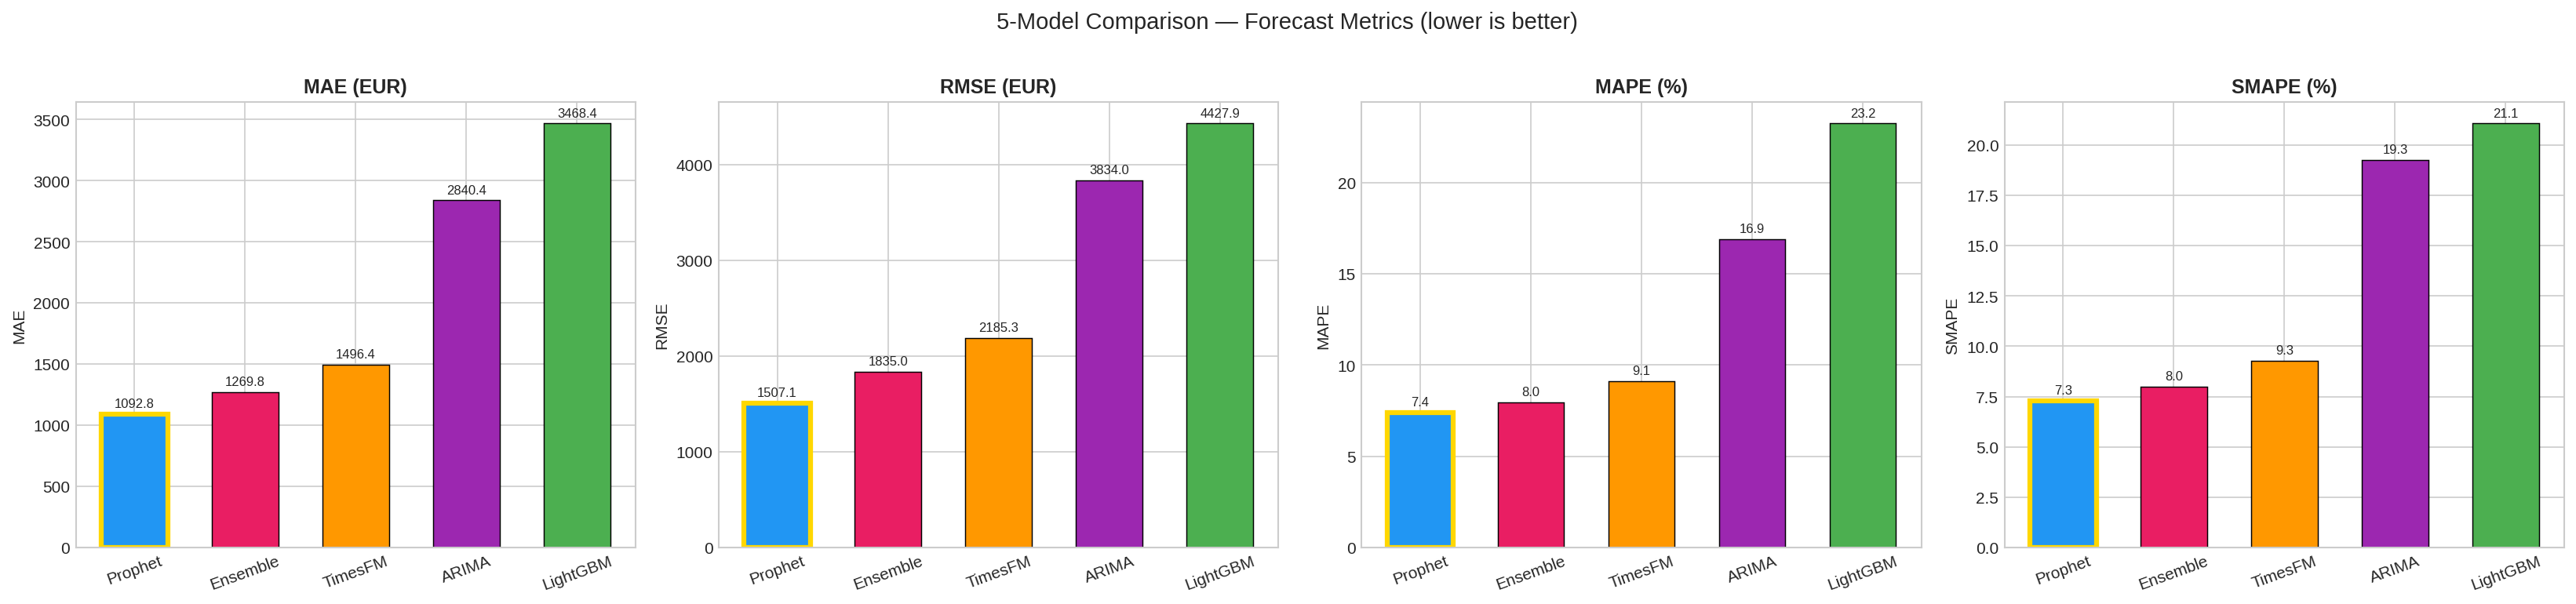
\includegraphics[width=0.85\textwidth]{figures/comparison_5model_metrics.png}
    \caption{Overall forecast metrics comparison across all five models (lower is better for error metrics). Prophet leads all accuracy metrics.}
    \label{fig:metrics}
\end{figure}

\begin{figure}[H]
    \centering
    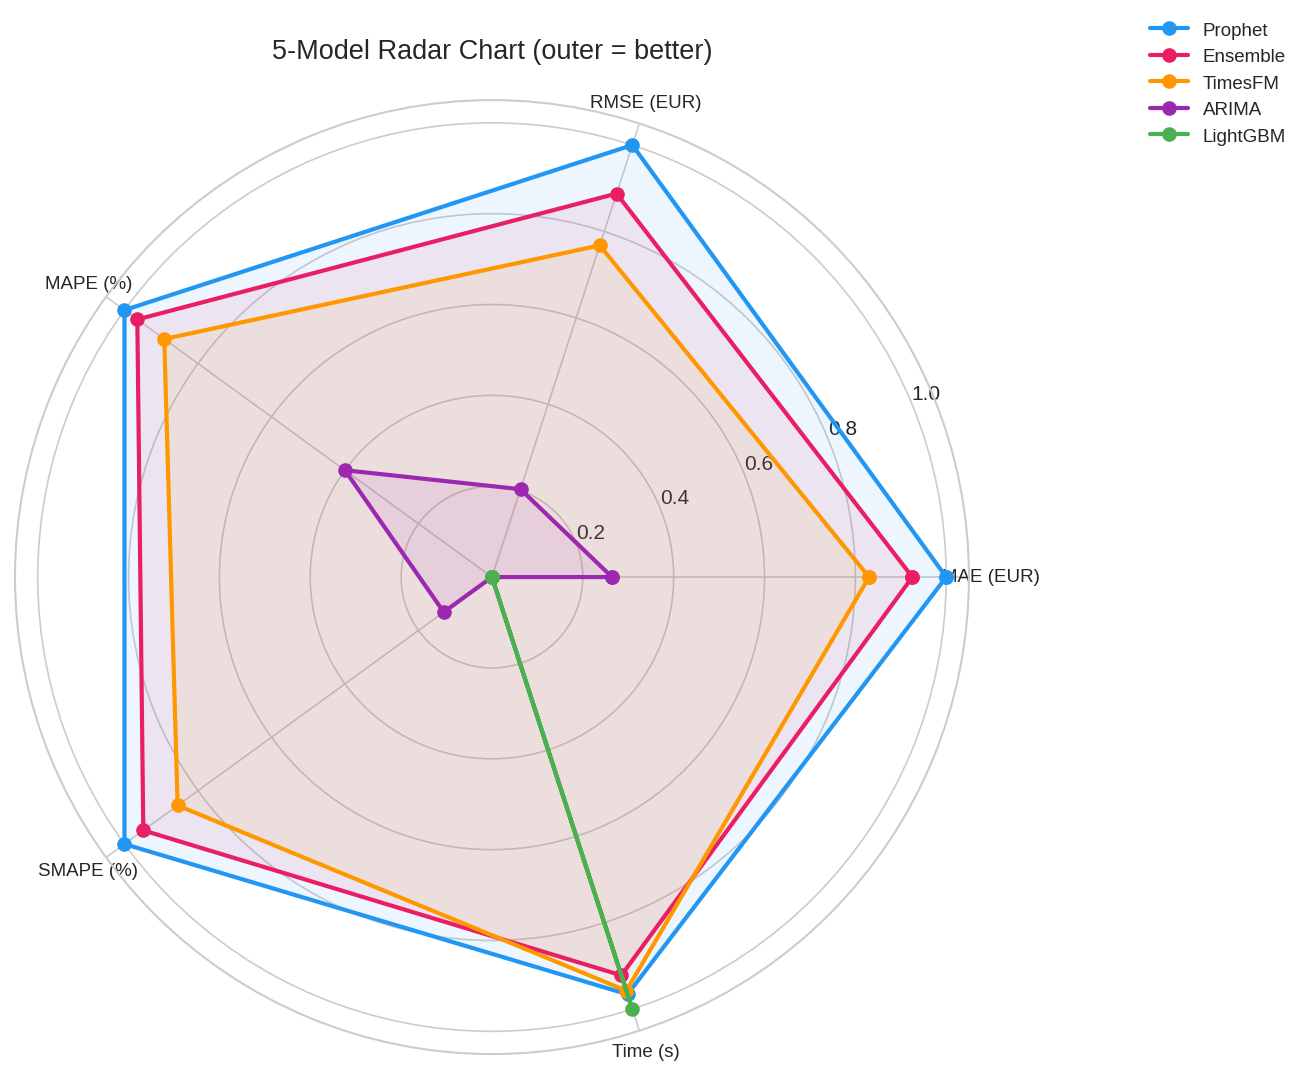
\includegraphics[width=0.85\textwidth]{figures/comparison_5model_radar.png}
    \caption{Multi-dimensional radar chart (outer = better). Prophet and Ensemble occupy the largest area, with TimesFM as a strong third.}
    \label{fig:radar}
\end{figure}

\subsection{Per-Country Performance}

\begin{table}[H]
\caption{Per-country MAE (\texteuro) with winner per market (synthetic data).}
\setlength{\tabcolsep}{8pt}
\renewcommand{\arraystretch}{1.4}
\begin{tabular}{l l l l l l}
\toprule
 & \textbf{ARIMA} & \textbf{Prophet} & \textbf{LGBM} & \textbf{TimesFM} & \textbf{Ensemble} \\
\midrule
BE & 1,873 & \textbf{726} & 2,140 & 1,024 & 811 \\
DE & 3,095 & \textbf{1,152} & 4,907 & 2,433 & 2,186 \\
ES & 2,318 & \textbf{1,154} & 3,731 & 1,252 & 1,171 \\
FR & 4,484 & \textbf{1,155} & 4,430 & 1,865 & 1,678 \\
IT & 5,142 & \textbf{1,017} & 2,246 & 1,492 & 1,017 \\
NL & 1,910 & 1,086 & 3,846 & 934 & \textbf{929} \\
PT & 1,473 & 961 & 1,563 & \textbf{876} & 876 \\
UK & 2,430 & \textbf{1,491} & 4,884 & 2,096 & 1,491 \\
\bottomrule
\end{tabular}
\end{table}

Prophet dominates 6 of 8 markets. The Ensemble wins Netherlands where the optimized weight ($w\!=\!0.18$) heavily favours TimesFM. TimesFM wins Portugal-the newest market with shortest history-validating foundation models for cold-start scenarios.

\subsection{Ensemble Weight Analysis}

\begin{table}[H]
\caption{Optimized ensemble weights (Prophet:TimesFM) per country.}
\setlength{\tabcolsep}{16pt}
\renewcommand{\arraystretch}{1.4}
\begin{tabular}{l l l l}
\toprule
\textbf{Country} & \textbf{$w$ (Prophet)} & \textbf{$1\!-\!w$ (TimesFM)} & \textbf{Dominance} \\
\midrule
IT & 1.00 & 0.00 & Prophet only \\
UK & 1.00 & 0.00 & Prophet only \\
BE & 0.56 & 0.44 & Balanced \\
ES & 0.24 & 0.76 & TimesFM-leaning \\
FR & 0.22 & 0.78 & TimesFM-leaning \\
NL & 0.18 & 0.82 & TimesFM-dominant \\
DE & 0.14 & 0.86 & TimesFM-dominant \\
PT & 0.00 & 1.00 & TimesFM only \\
\bottomrule
\end{tabular}
\end{table}

The learned weights encode market intelligence: mature markets with established promotional patterns (IT, UK) favour Prophet exclusively, while emerging markets (PT) rely entirely on TimesFM's pre-trained temporal knowledge. Average weighting: Prophet 42\%, TimesFM 58\%.

\subsection{Analysis and Discussion}

\textbf{Why Prophet Wins:} Prophet's superiority stems from encoding domain knowledge as multiplicative regressors-\texttt{promotion\_flag} directly signals Q4 demand spikes, and \texttt{covid\_period\_flag} models the 2020--2021 regime change. Its near-zero mean residual confirms unbiased predictions versus TimesFM's systematic under-prediction during promotional weeks. Two simple binary features outperform 26 engineered ones.

\textbf{Why LightGBM Fails:} Despite 26 features, LightGBM ranks last due to its recursive multi-step strategy. Feature importance reveals \texttt{lag\_1} dominates ($\sim$60\% of splits), creating a prediction$\rightarrow$lag$\rightarrow$prediction feedback loop where errors compound by step 12. Prophet and TimesFM avoid this by forecasting the entire horizon simultaneously. This failure pattern is consistent with findings from the M5 forecasting competition~\cite{makridakis2020m5}.

This is likely a data/modeling issue rather than a code bug. With only $\sim$103 effective training rows per country and a recursive 12-step forecast strategy, LightGBM (a tabular gradient booster) simply does not have enough data to learn robust lag patterns. Prophet and the ensemble handle small-data time-series much better by design-Prophet through decomposition priors, and TimesFM through its 400B+ pre-training corpus.

\textbf{Why LightGBM looks odd on the radar chart:} The radar normalization uses $1 - (value - min) / (max - min)$, mapping the best (lowest error) to 1.0 and worst to 0.0. LightGBM has the worst error metrics across all axes but is by far the fastest model. On the radar chart this means 4 of 5 axes collapse to the center (radius~$\approx$~0) and only the Time axis extends to the rim. The ``polygon'' degenerates into a single spoke-a straight line from center to the outer edge and back. Thought it appeared to be a plotting bug initially, but it correctly reflects how extreme LightGBM's underperformance is relative to the other models.

\textbf{Foundation Model Positioning:} TimesFM achieves second place among individual models \textit{without any training, regressors, or configuration}-outperforming both ARIMA (trained) and LightGBM (trained, 26 features). Though there was no much effort the result is remarkably strong. It validates foundation models as the strongest zero-configuration option, particularly useful for cold-start markets where you have no historical promotional calendars to encode.

\begin{figure}[H]
    \centering
    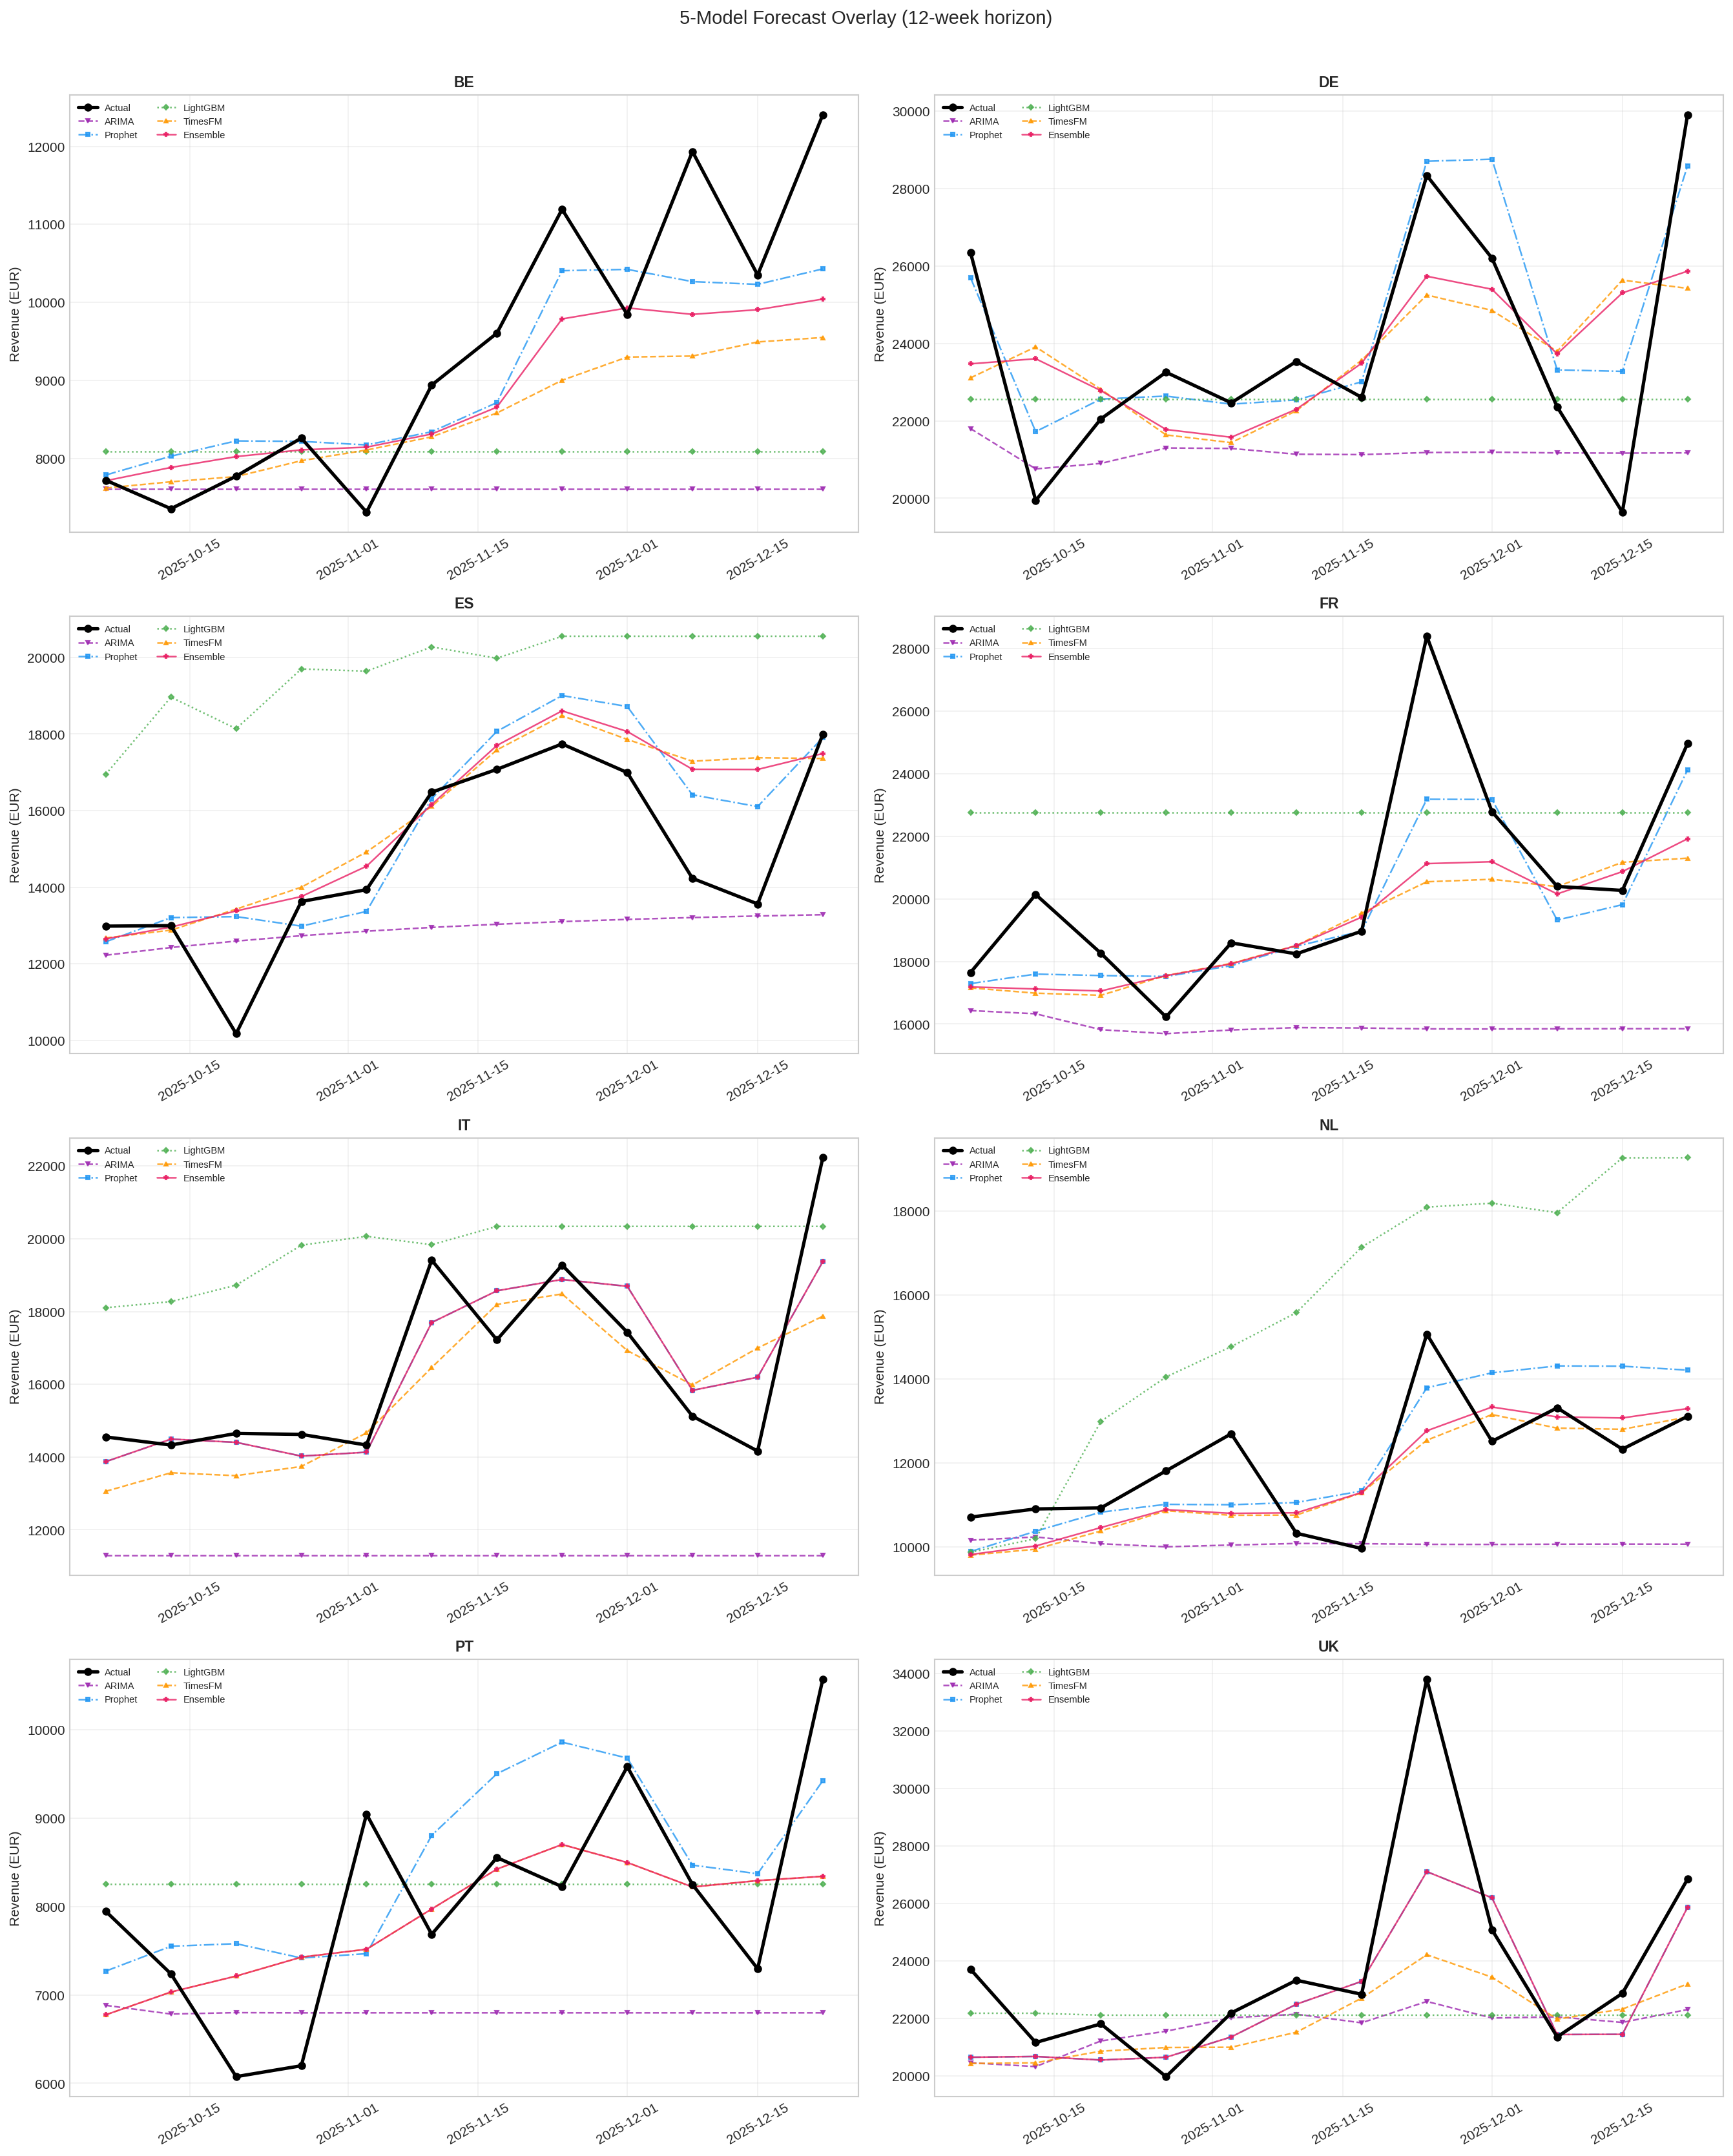
\includegraphics[width=0.85\textwidth]{figures/comparison_5model_forecast_overlay.png}
    \caption{Forecast overlay: all 5 models vs actual values. Prophet and Ensemble track actuals most closely during Q4 promotional peaks.}
    \label{fig:overlay}
\end{figure}

\begin{figure}[H]
    \centering
    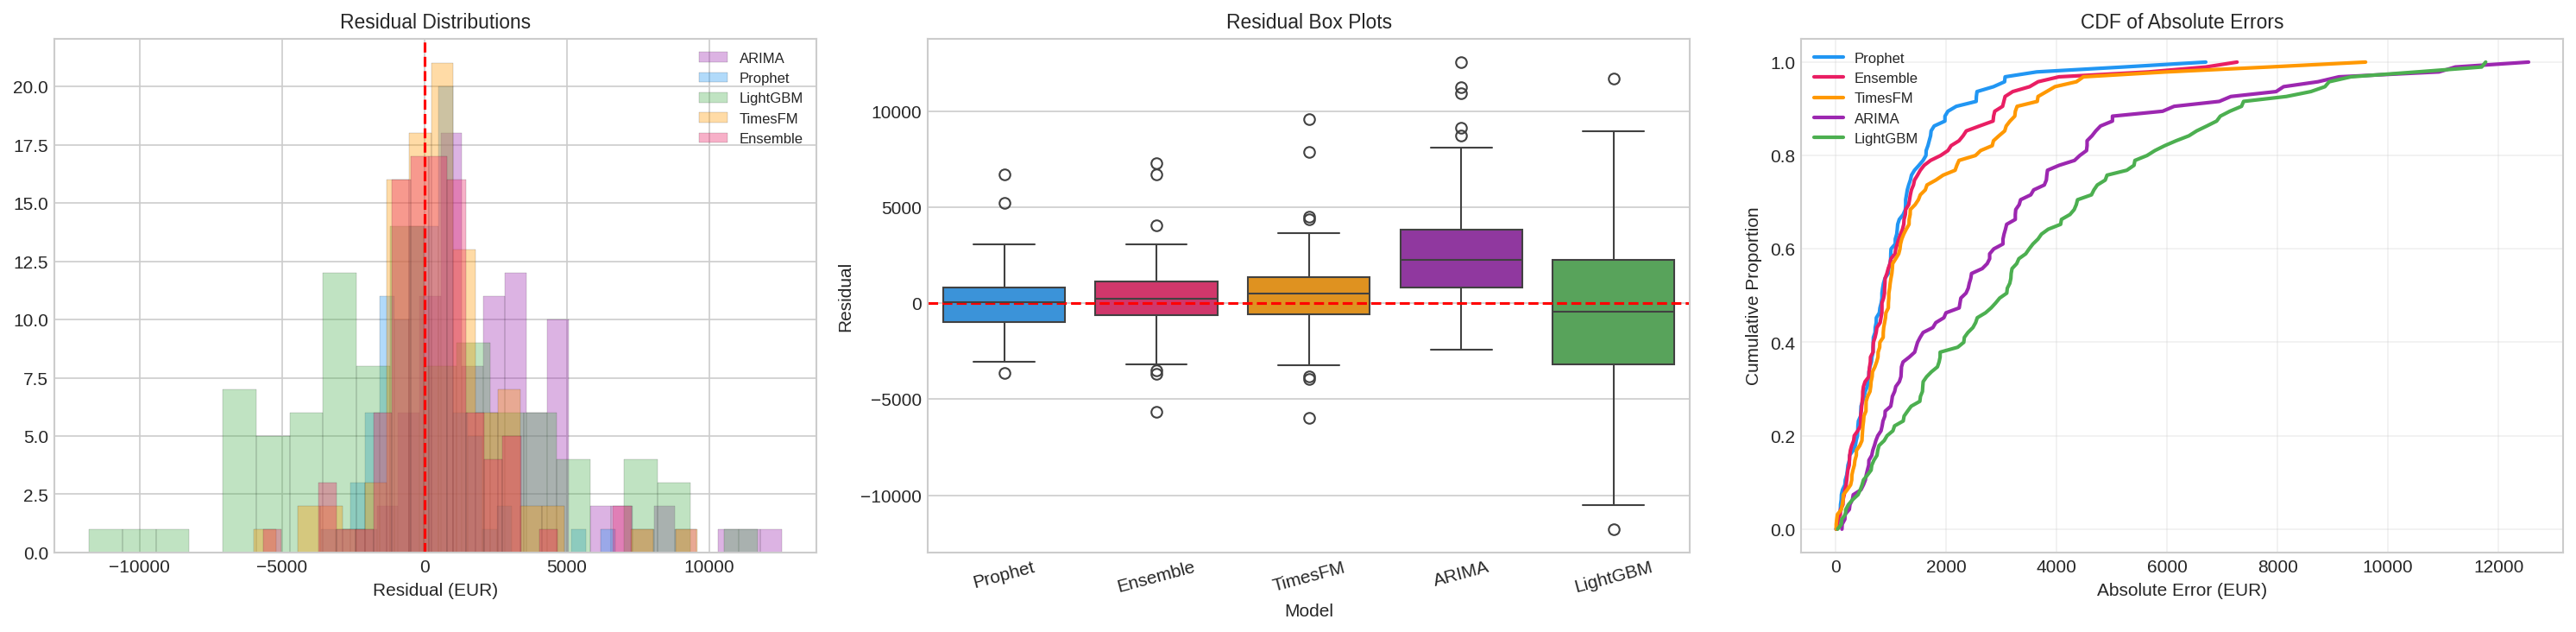
\includegraphics[width=0.85\textwidth]{figures/comparison_5model_residuals.png}
    \caption{Residual analysis: distribution overlap, box plots, and CDF of absolute errors. Prophet has the tightest distribution centred near zero.}
    \label{fig:residuals}
\end{figure}

\subsection{Production Recommendation}

\begin{table}[H]
\caption{Recommended three-tier production forecasting architecture.}
\setlength{\tabcolsep}{16pt}
\renewcommand{\arraystretch}{1.4}
\begin{tabular}{l l l l}
\toprule
\textbf{Tier} & \textbf{Model} & \textbf{MAPE} & \textbf{Use Case} \\
\midrule
1 & Prophet & 7.40\% & Mature markets with promo calendars \\
2 & Ensemble & 7.95\% & Multi-market adaptive system \\
3 & TimesFM & 9.11\% & Cold-start, scaling, rapid POC \\
\bottomrule
\end{tabular}
\end{table}

\textbf{Ongoing Work:} More experiments are in progress to infuse real operational data-including customer feedback of varying length, typos, and edge-case promotional patterns-to further validate these models before completing the integration into the Company's actual forecasting system.

% =============================================================================
% STUDY C: SENTIMENT ANALYSIS (~5 pages)
% =============================================================================
\section{Study C: Multilingual Sentiment Analysis}

\subsection{Objective}
The goal here was to find the best deep learning architecture for classifying customer review sentiment across 7 European languages (English, French, German, Spanish, Italian, Dutch, Portuguese). I wanted to compare native multilingual processing versus a translate-then-classify approach, and I needed a methodology that reveal differences between models-which turned out to be harder than expected.

\subsection{Datasets}

I ran several mini experiments with different model candidates before settling on the final 8 architectures reported here. Early on, I tested smaller RNN variants and a vanilla CNN-based classifier, but they were clearly outclassed by transformers on even basic data, so I dropped them from the formal comparison.

\begin{table}[H]
\caption{Dataset characteristics across experimental phases (synthetic data).}
\setlength{\tabcolsep}{22pt}
\renewcommand{\arraystretch}{1.4}
\begin{tabular}{l l l}
\toprule
\textbf{Attribute} & \textbf{Phase 1} & \textbf{Phase 2} \\
\midrule
Total reviews & 550 & 1,800 \\
Languages & 7 & 7 \\
Classes & 3 (Pos/Neu/Neg) & 3 (Pos/Neu/Neg) \\
Difficulty & Low (clear signals) & High (ambiguous) \\
Test samples & 83 & 270 \\
\bottomrule
\end{tabular}
\end{table}

Both datasets are synthetically generated to replicate Trustpilot-style review patterns without exposing any actual customer feedback. The Phase~1 dataset was initially inspired by a minimal portion of real Trustpilot reviews-I studied the structure, length distribution, and language mix of actual reviews, then generated synthetic equivalents that preserved those characteristics without using any explicit content or context from the originals.

\subsection{Phase 1: Baseline Validation (4 Architectures)}

Four architectures were evaluated on the structured dataset to confirm implementation correctness:
\begin{itemize}[leftmargin=*,noitemsep,topsep=2pt]
    \item \textbf{Bi-LSTM:} Embedding $\rightarrow$ Bidirectional LSTM $\rightarrow$ Dense ($\sim$500K params)~\cite{hochreiter1997long}
    \item \textbf{Bi-GRU:} Embedding $\rightarrow$ Bidirectional GRU $\rightarrow$ Dense ($\sim$375K params)
    \item \textbf{BERT:} \texttt{bert-base-multilingual-cased}~\cite{devlin2019bert} $\rightarrow$ [CLS] $\rightarrow$ Linear (177.9M params)
    \item \textbf{DistilBERT:} \texttt{distilbert-base-multilingual-cased} $\rightarrow$ [CLS] $\rightarrow$ Linear (135.3M params)
\end{itemize}

All four achieved 100\% accuracy. This made me skepitical about overfitting related issues, but I found the Phase~1 data was simply too clean-sentiment signals were unambiguous, sentences were short and grammatically correct, and there was no sarcasm or mixed sentiment. Every model could handle it trivially. So I tried the Phase~2 approach.

Key differentiator from Phase~1: transformers train 3--7$\times$ faster than RNNs despite 300--500$\times$ more parameters due to pre-trained representations (BERT reaches 84\% validation accuracy at epoch 1 vs.\ LSTM starting at $\sim$50\%).

\begin{figure}[H]
    \centering
    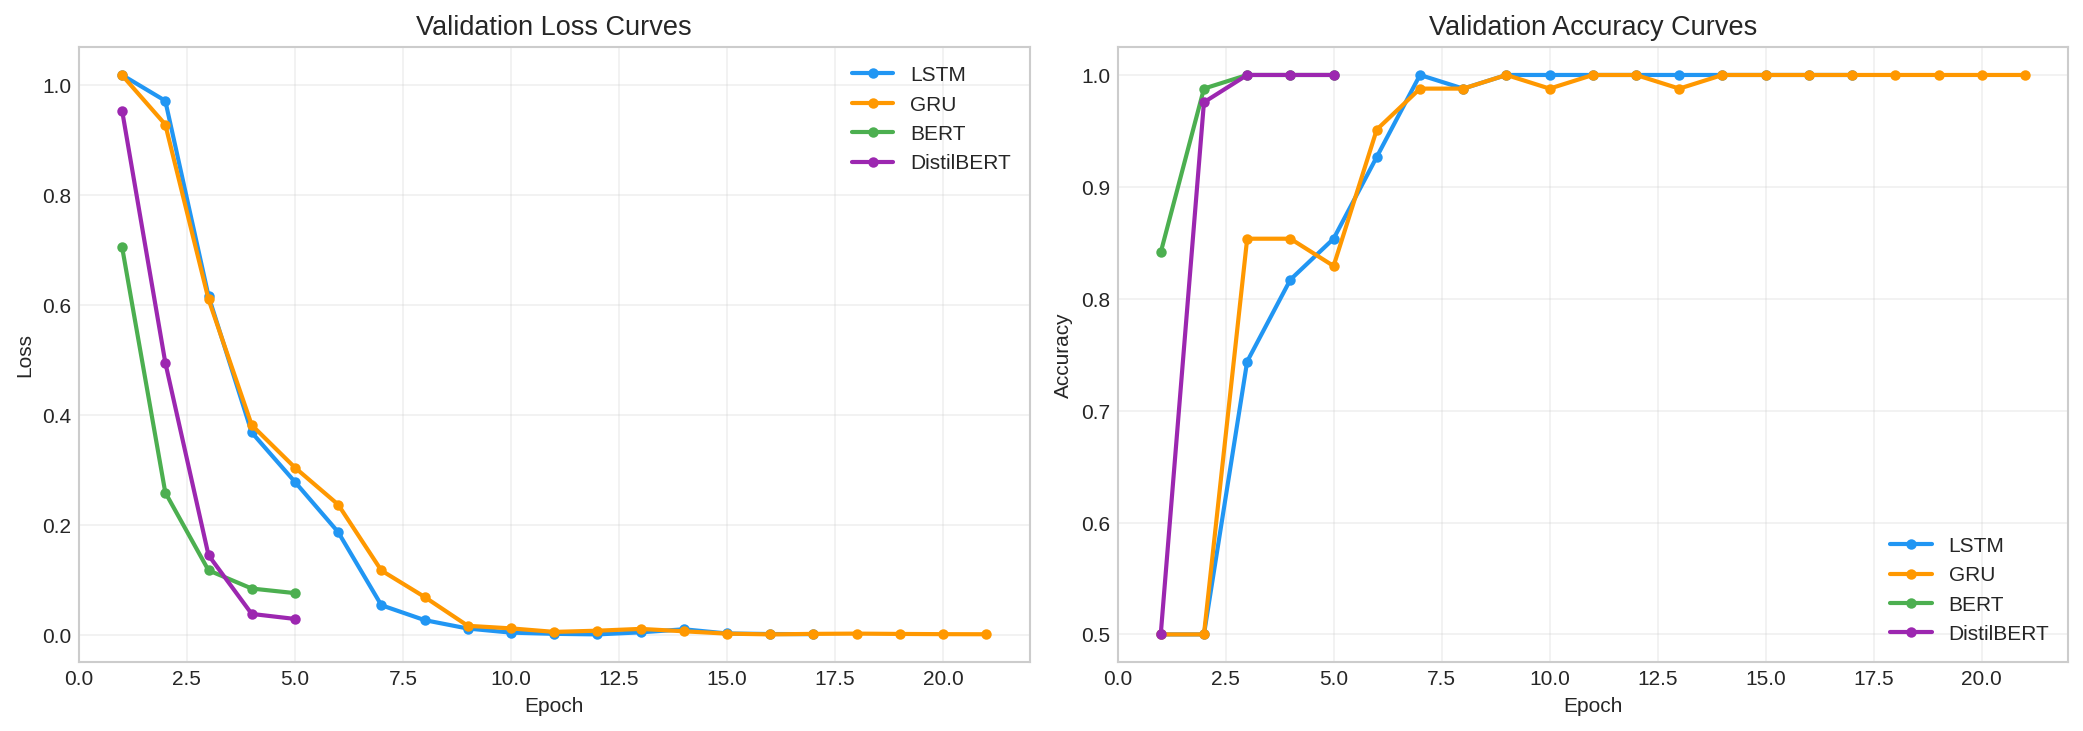
\includegraphics[width=0.85\textwidth]{figures/phase1_training_curves.png}
    \caption{Phase 1: Training convergence curves. Transformers (BERT, DistilBERT) converge significantly faster due to pre-trained representations.}
    \label{fig:phase1_training}
\end{figure}

\subsection{Phase 2: Challenge Dataset (4 Advanced Architectures)}

To do effective analysis and find the best model for actual production reviews, I needed data that would break models-not confirm them. I built a custom Python-based tooling pipeline to generate ``hard'' synthetic reviews: text with sarcasm (``Great, another delayed shipment. Just what I needed.''), mixed sentiment within a single review, rating-label mismatches, and typos typical of real user input. The generator produced 1,800 reviews across 7 languages that are closer to what real Trustpilot feedback looks like, without using any explicit content from actual reviews.

Two processing approaches were compared on this harder dataset:

\textbf{Approach A - Native Multilingual:}
\begin{itemize}[leftmargin=*,noitemsep,topsep=2pt]
    \item BERT+BiLSTM: \texttt{bert-base-multilingual-cased} $\rightarrow$ BiLSTM $\rightarrow$ Dense~\cite{nkhata2025finetuning}
    \item XLM-RoBERTa: \texttt{xlm-roberta-base}~\cite{conneau2020unsupervised} $\rightarrow$ [CLS] $\rightarrow$ Dense
\end{itemize}

\textbf{Approach B - Translate-then-Classify} (Google Translate $\rightarrow$ English):
\begin{itemize}[leftmargin=*,noitemsep,topsep=2pt]
    \item BERT+BiLSTM: \texttt{bert-base-uncased} $\rightarrow$ BiLSTM $\rightarrow$ Dense
    \item RoBERTa: \texttt{roberta-base}~\cite{liu2019roberta} $\rightarrow$ [CLS] $\rightarrow$ Dense
\end{itemize}

Training configuration: max sequence 128, batch 32, lr 2e-5, AdamW optimizer, early stopping (patience 3), NVIDIA T4 GPU.

\begin{table}[H]
\caption{Phase 2 results on hard dataset (1,800 reviews, 270 test, synthetic data).}
\setlength{\tabcolsep}{10pt}
\renewcommand{\arraystretch}{1.4}
\begin{tabular}{l l l l l l}
\toprule
\textbf{Model} & \textbf{Approach} & \textbf{Accuracy} & \textbf{F1} & \textbf{AUC} & \textbf{Time} \\
\midrule
BERT+BiLSTM & Multilingual & 97.78\% & 0.979 & 0.998 & 269s \\
XLM-RoBERTa & Multilingual & 98.15\% & 0.981 & 1.000 & 192s \\
BERT+BiLSTM & English & \textbf{99.63\%} & \textbf{0.996} & 1.000 & 122s \\
RoBERTa & English & \textbf{99.63\%} & \textbf{0.996} & \textbf{1.000} & 139s \\
\bottomrule
\end{tabular}
\end{table}

\begin{figure}[H]
    \centering
    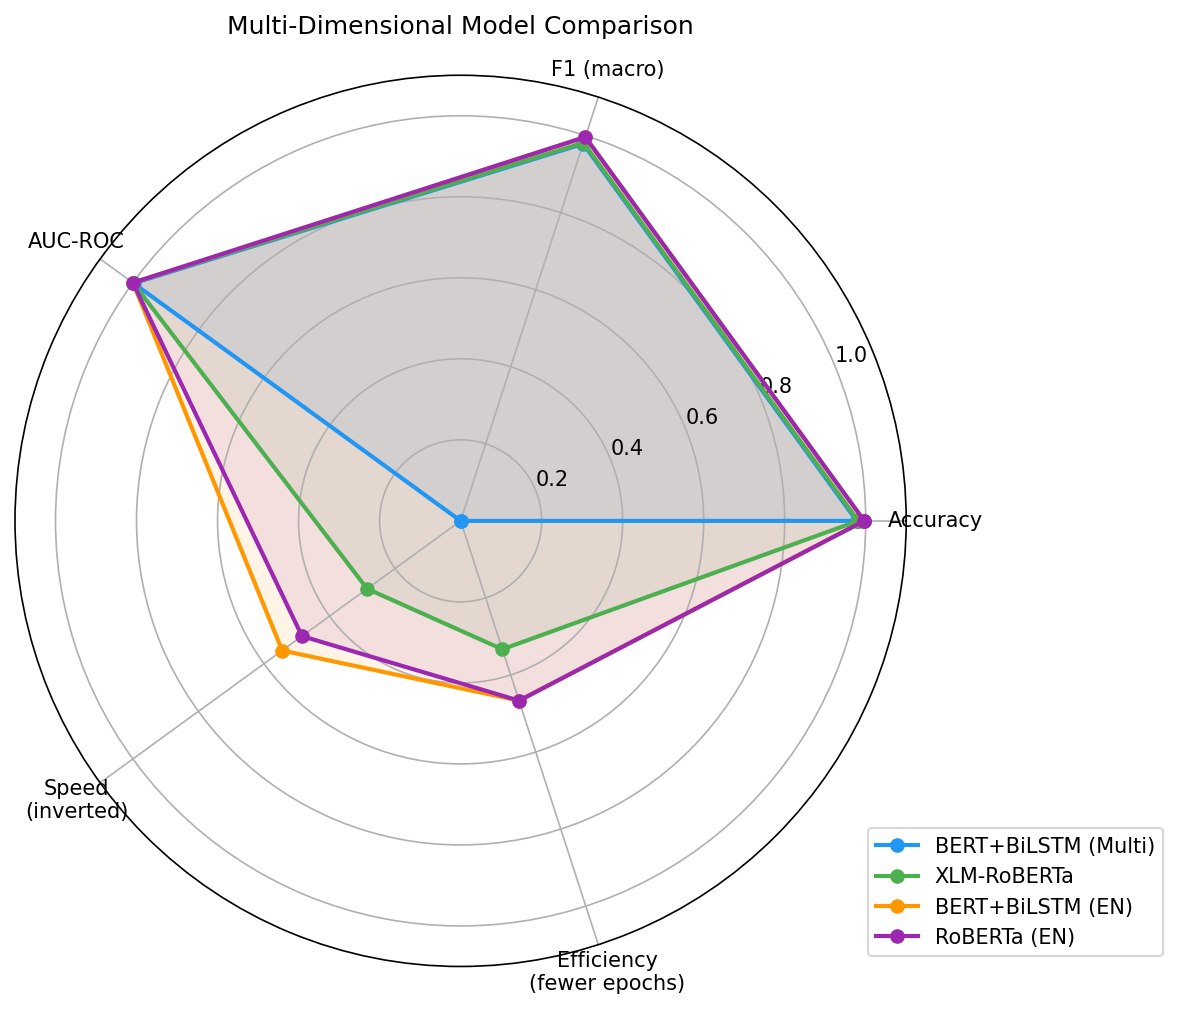
\includegraphics[width=0.85\textwidth]{figures/phase2_radar.png}
    \caption{Phase 2: Multi-metric radar comparison. Translated models (outer boundary) dominate across all dimensions including accuracy, F1, AUC, and training speed.}
    \label{fig:phase2_radar}
\end{figure}

\subsection{Approach-Level Comparison}

\begin{table}[H]
\caption{Aggregated comparison: Multilingual vs.\ Translated approaches.}
\setlength{\tabcolsep}{16pt}
\renewcommand{\arraystretch}{1.4}
\begin{tabular}{l l l l}
\toprule
\textbf{Metric} & \textbf{Multilingual} & \textbf{Translated} & \textbf{$\Delta$} \\
\midrule
Avg. Accuracy & 97.96\% & \textbf{99.63\%} & +1.67\% \\
Avg. F1 (macro) & 0.980 & \textbf{0.996} & +0.016 \\
Avg. AUC-ROC & 0.999 & \textbf{1.000} & +0.001 \\
Avg. Training Time & 230.3s & \textbf{130.5s} & $-$43\% \\
\bottomrule
\end{tabular}
\end{table}

\begin{figure}[H]
    \centering
    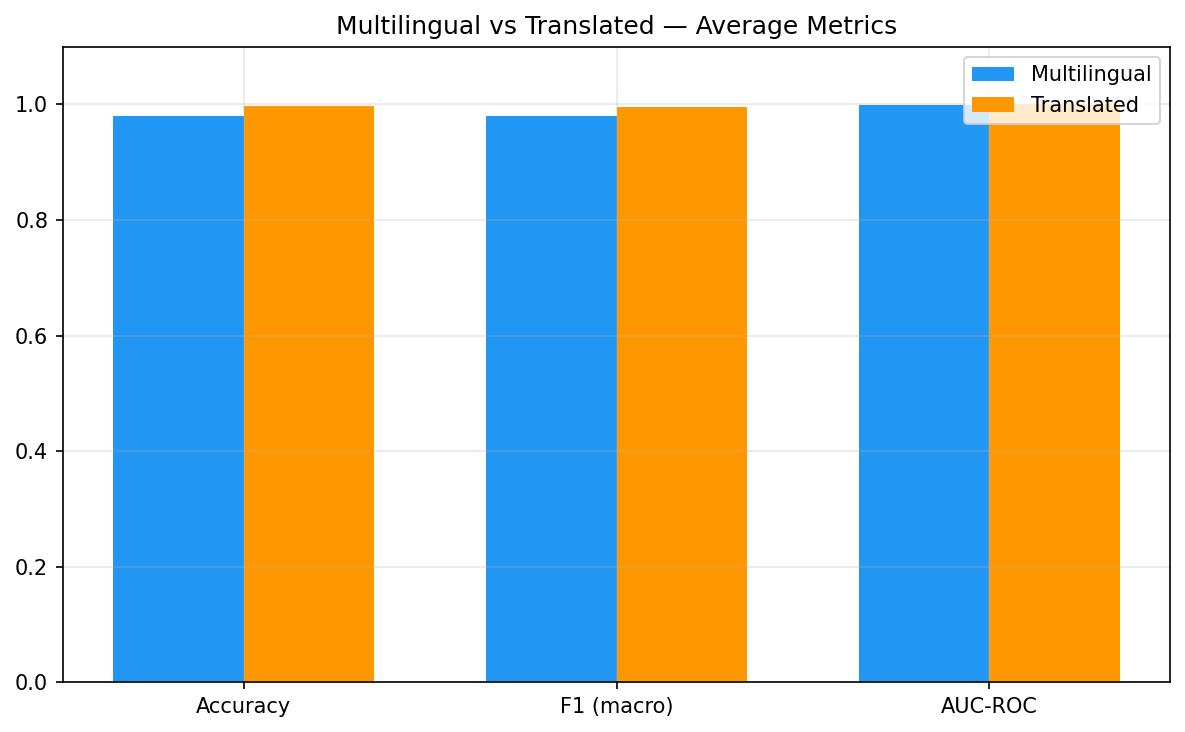
\includegraphics[width=0.85\textwidth]{figures/approach_summary.png}
    \caption{Approach-level performance summary: translated models achieve superior accuracy and 43\% faster training across all metrics.}
    \label{fig:approach}
\end{figure}

\subsection{Analysis and Discussion}

\textbf{Translation as Feature Engineering:} I found that translate-then-classify effectively normalises linguistic variation-morphological complexity, word order differences, and idiomatic expressions-into a standardised representation that English-optimised models process more effectively. The tradeoff is real though: this introduces a dependency on translation APIs (latency, cost, availability) that may not be acceptable for all use cases.

\textbf{BERT+BiLSTM on Short Text:} I specifically included the BERT+BiLSTM hybrid because Nkhata et al.~\cite{nkhata2025finetuning} reported strong results on long movie reviews. On our short customer reviews ($\sim$30--50 words), it does \textit{not} outperform standard transformer fine-tuning. The additional BiLSTM layer adds computational overhead without capturing meaningful sequential patterns in text of this length. This was a useful negative result.

\textbf{Error Analysis:} RoBERTa (EN) commits only 1 misclassification (neutral$\rightarrow$positive) out of 270 test samples. Multilingual models exhibit 5--6 errors, predominantly in the negative$\leftrightarrow$positive confusion zone where ambiguous sentiment markers in non-English languages are better resolved after translation normalisation.

\textbf{Ongoing Work:} More experiments are in progress infusing real customer data-reviews with varying lengths, actual typos, and genuine sarcasm-to further validate these findings before completing the integration into the Company's production sentiment monitoring system.

\begin{figure}[H]
    \centering
    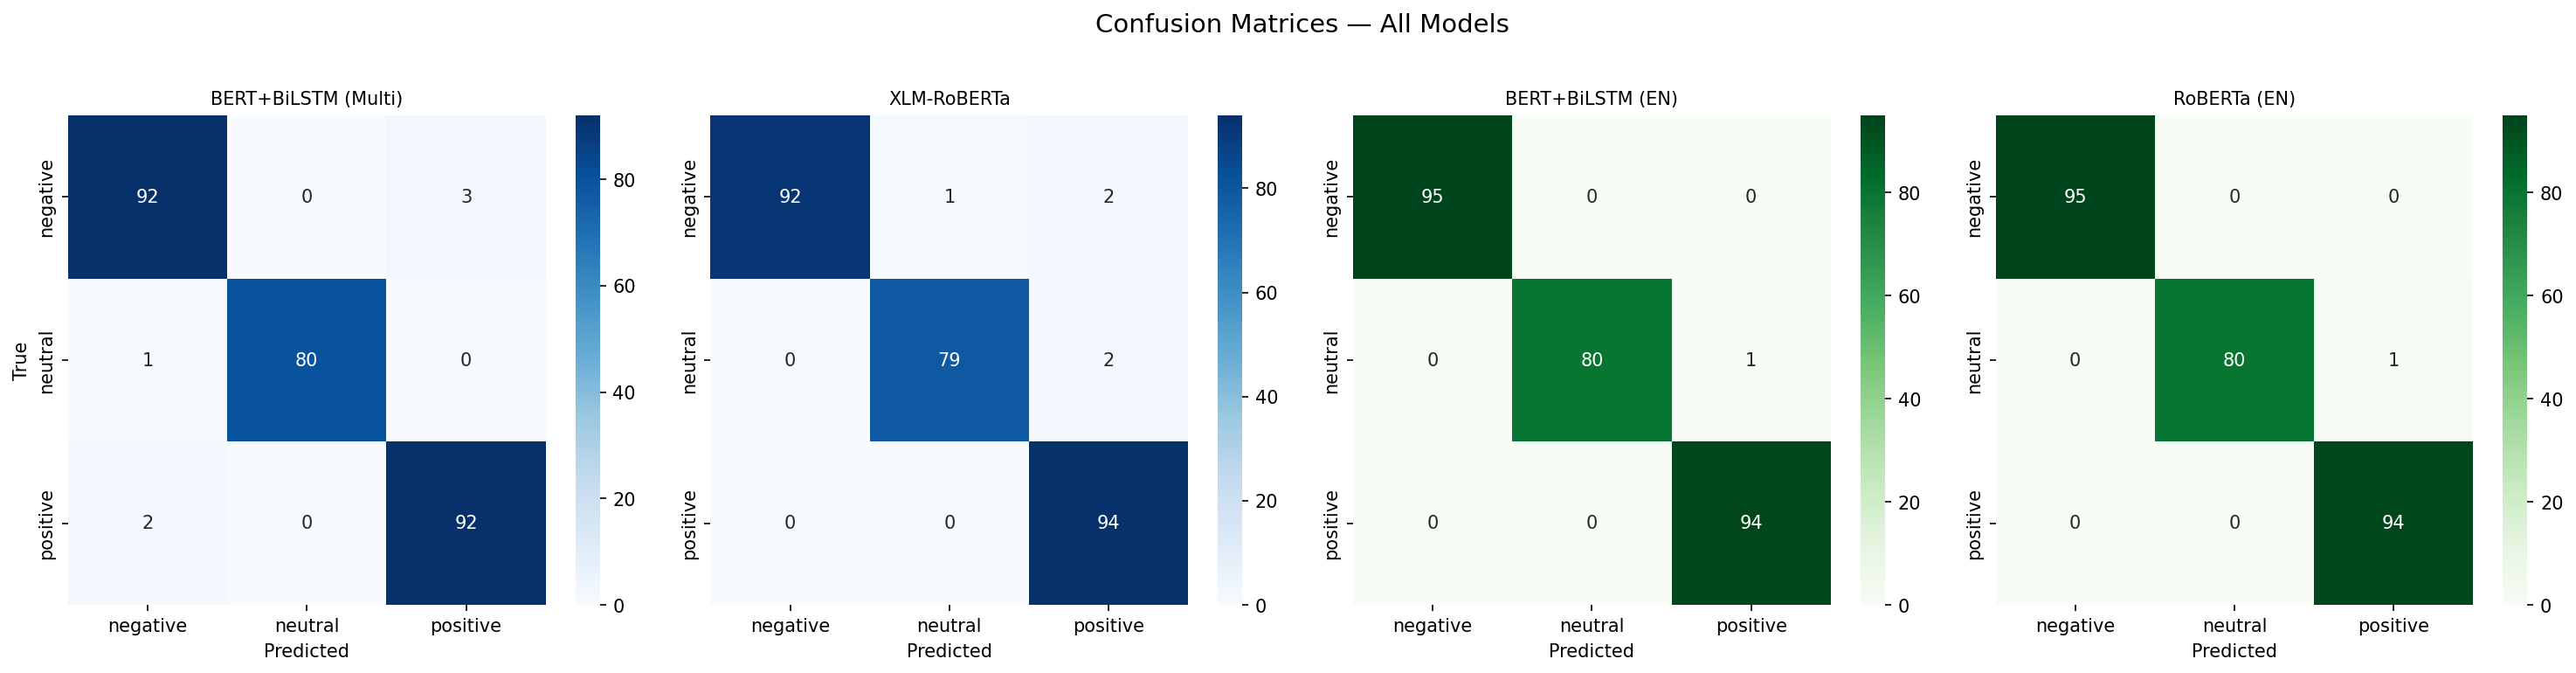
\includegraphics[width=0.85\textwidth]{figures/phase2_confusion_matrices.png}
    \caption{Confusion matrices: translated models show near-perfect classification with minimal neutral$\leftrightarrow$polar confusion.}
    \label{fig:confusion}
\end{figure}

\subsection{Production Architecture}

\begin{table}[H]
\caption{Recommended two-tier sentiment deployment architecture.}
\setlength{\tabcolsep}{6pt}
\renewcommand{\arraystretch}{1.4}
\begin{tabular}{l l l l}
\toprule
\textbf{Tier} & \textbf{Model} & \textbf{Accuracy} & \textbf{Use Case} \\
\midrule
Batch & RoBERTa (EN) + Translation & 99.63\% & Overnight reports, dashboards \\
Real-time & XLM-RoBERTa & 98.15\% & Instant alerts, no API dependency \\
\bottomrule
\end{tabular}
\end{table}

% =============================================================================
% STUDY D: CONVERSATIONAL AI AGENT (~5 pages)
% =============================================================================
\section{Study D: Conversational AI Agent}

\subsection{Objective}
Design, deploy, and quantitatively evaluate a domain-specific conversational AI agent that trains pharmaceutical sales representatives in the SPIN Selling methodology~\cite{rackham1988spin}-a structured questioning technique for consultative sales involving Situation, Problem, Implication, and Need-payoff questions.

\subsection{Platform Selection: Dead Ends and Final Choice}

I initially tried building this on Vertex AI Agent Builder. It worked, but it was comparatively complex for what I needed, and critically, it only exposed API access to the agent-no built-in chat interface for sales reps to actually use during training sessions. I spent time investigating whether I could try on a separate Google Chat Bot as the frontend, but the integration complexity was disproportionate to the value. Instead, I pivoted to Google ADK which comes with a Web UI out of the box and deploys cleanly to Cloud Run. This ended up being the right solution-the ADK Web UI gave us an immediately usable coaching interface without building a custom frontend.

\subsection{Technical Architecture}

\begin{table}[H]
\caption{Agent system architecture and technology stack.}
\setlength{\tabcolsep}{36pt}
\renewcommand{\arraystretch}{1.4}
\begin{tabular}{l l}
\toprule
\textbf{Component} & \textbf{Technology} \\
\midrule
LLM Model & Gemini 3.1 Flash Lite \\
Orchestration Framework & Google ADK (v0.3+) \\
RAG Knowledge Base & Custom JSON (keyword retrieval) \\
Session Management & ADK InMemorySessionService \\
Deployment & Google Cloud Run (serverless) \\
Container & Python 3.12 + Docker \\
API Security & Secret Manager (API key) \\
Auto-scaling & 0--3 instances \\
\bottomrule
\end{tabular}
\end{table}

\textbf{Model Selection Rationale:} Gemini 3.1 Flash Lite was selected for optimal balance of speed (3.1s average latency), cost (lowest per-token in Gemini family), quality (sufficient instruction-following for structured coaching), and context window (128K tokens for full conversation history).

\subsection{Agent Operational Modes}

The agent operates through three modes defined by a detailed system instruction:

\begin{enumerate}[leftmargin=*,noitemsep,topsep=2pt]
    \item \textbf{Teaching Mode:} Provides SPIN methodology guidance grounded in RAG-retrieved content from a curated knowledge base
    \item \textbf{Evaluation Mode:} Scores user-submitted sales pitches against SPIN criteria, identifying premature solutioning and suggesting restructured approaches
    \item \textbf{Role-Play Mode:} Simulates buyer personas (4 clinic types $\times$ 3 difficulty levels) with hidden pain points that users must uncover through proper SPIN questioning
\end{enumerate}

\subsection{Tool Architecture}

Four function-calling tools extend the agent beyond text generation:

\begin{table}[H]
\caption{Agent tools, invocation patterns, and purposes.}
\setlength{\tabcolsep}{16pt}
\renewcommand{\arraystretch}{1.4}
\begin{tabular}{l l l}
\toprule
\textbf{Tool} & \textbf{Called} & \textbf{Purpose} \\
\midrule
\texttt{search\_knowledge\_base} & 21/60 & RAG retrieval from training content \\
\texttt{evaluate\_spin\_message} & 10/60 & Score user pitches on SPIN criteria \\
\texttt{start\_roleplay} & 7/60 & Initialize buyer persona scenarios \\
\texttt{get\_coaching\_progress} & 2/60 & Track session performance metrics \\
(no tool - direct) & 20/60 & Respond from instruction context \\
\bottomrule
\end{tabular}
\end{table}

\subsection{RAG Implementation}

The knowledge base is a pre-processed JSON corpus with keyword-based relevance scoring, following Retrieval-Augmented Generation principles~\cite{lewis2020rag}:
\begin{itemize}[leftmargin=*,noitemsep,topsep=2pt]
    \item Word overlap scoring with section-title boosting ($\times$5)
    \item SPIN phase keyword matching ($+$10 per phase detected)
    \item Exact phrase matching ($+$20)
    \item Top-$k$ retrieval (default $k\!=\!5$)
\end{itemize}

A synthetic knowledge base was used exclusively for evaluation. In production deployment, the RAG layer connects to internal operational data via the same retrieval interface.

\subsection{Cloud Deployment}

\begin{figure}[H]
    \centering
    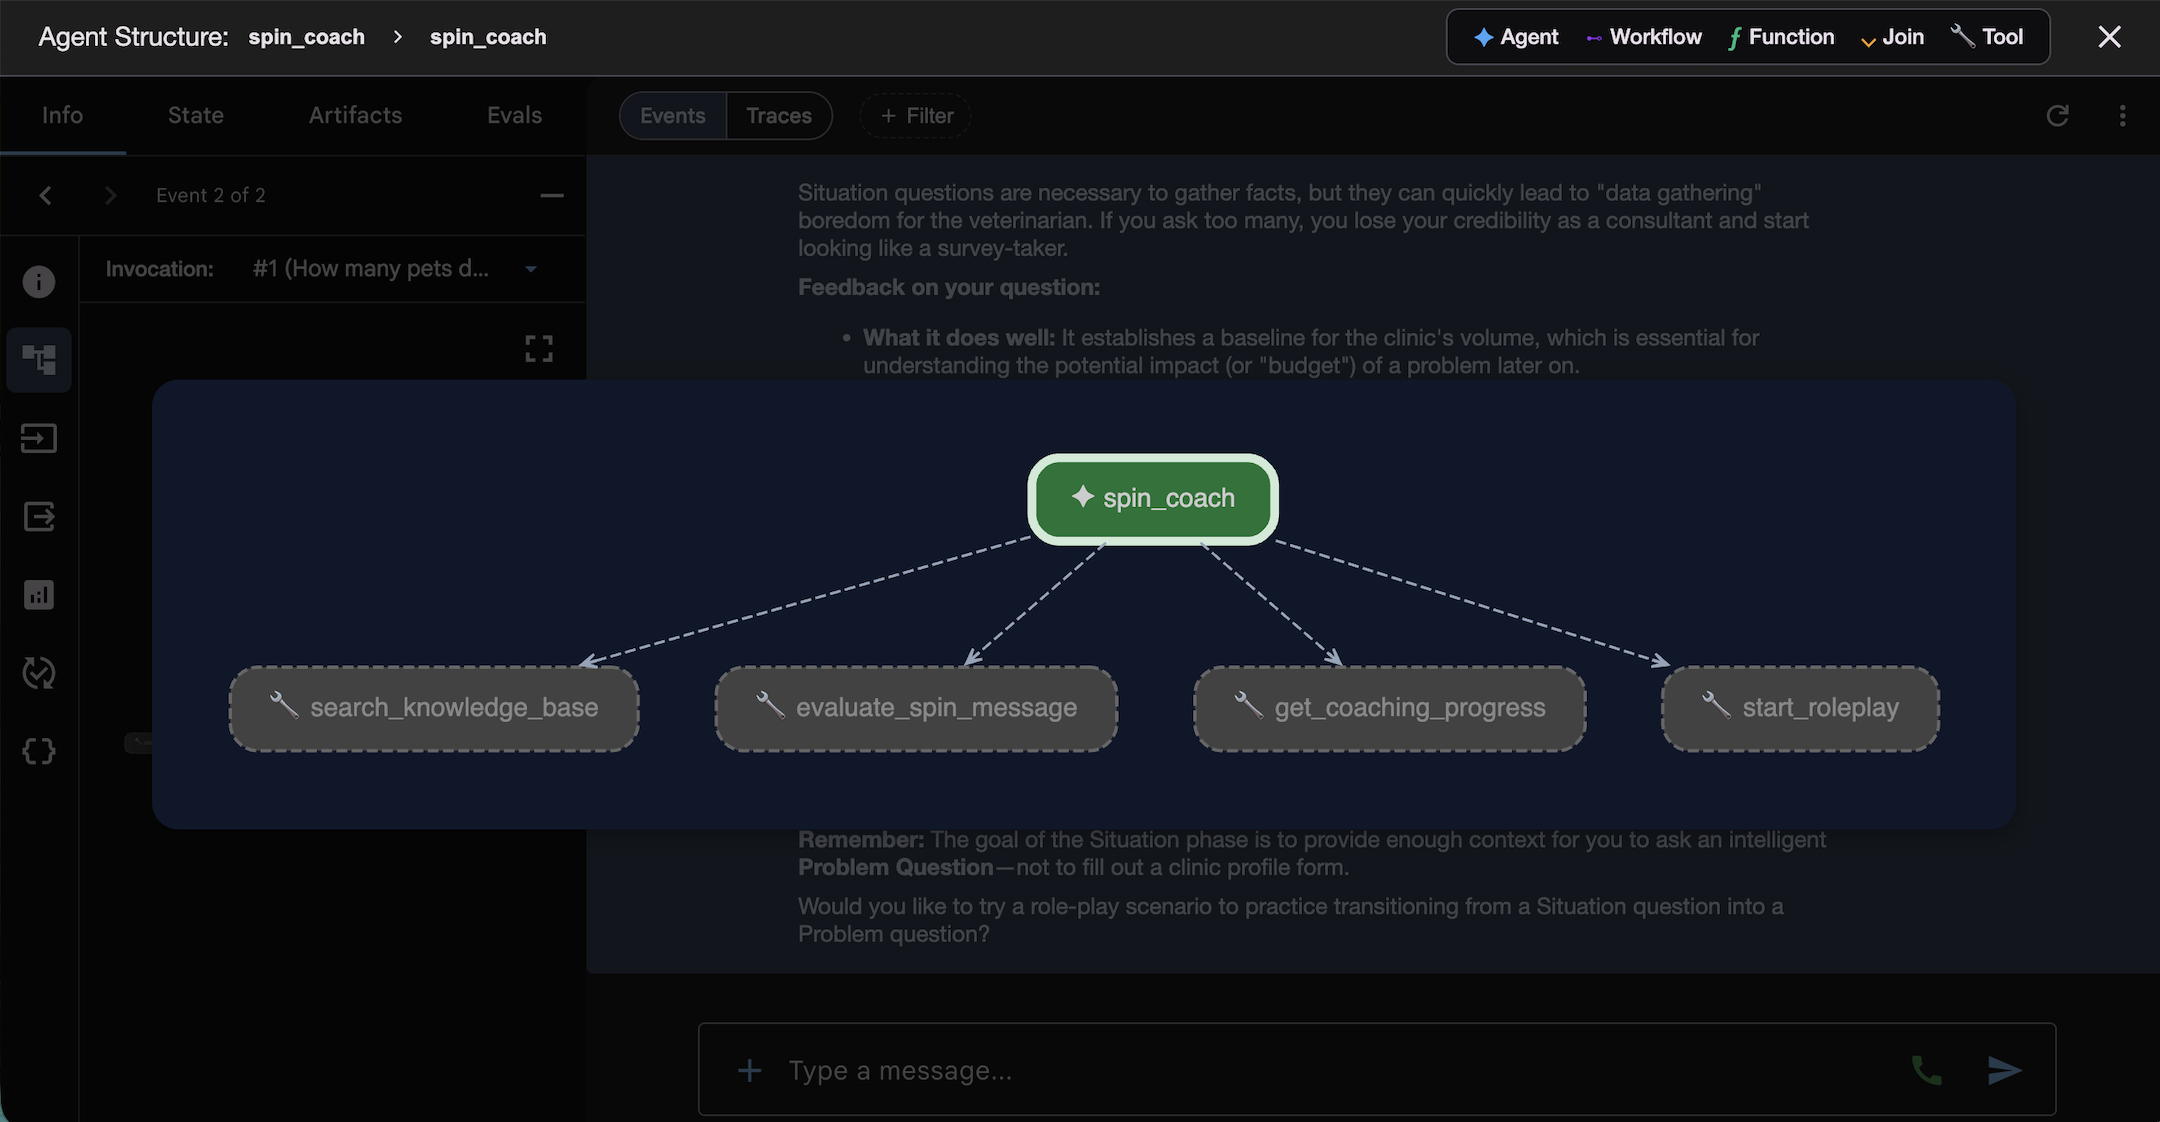
\includegraphics[width=0.85\textwidth]{figures/agent_cloud_run_deploy.png}
    \caption{Agent deployed on Google Cloud Run: serverless container with ADK Web UI, auto-scaling 0--3 instances based on demand.}
    \label{fig:cloudrun}
\end{figure}

Deployment configuration: Python 3.12 Docker container, 512~MB RAM, 1~vCPU per instance, API key secured via Secret Manager, ADK Web UI exposed on port 8080, unauthenticated access for internal evaluation.

\subsection{Evaluation Methodology}

A three-layer automated evaluation framework comprising 60 curated test cases across 6 categories:

\begin{table}[H]
\caption{Test case categories targeting different agent capabilities.}
\setlength{\tabcolsep}{16pt}
\renewcommand{\arraystretch}{1.4}
\begin{tabular}{l l l}
\toprule
\textbf{Category} & \textbf{Cases} & \textbf{Tests} \\
\midrule
SPIN Teaching & 12 & Methodology knowledge depth \\
SPIN Evaluation & 10 & Feedback quality on pitches \\
Role-Play & 8 & Persona consistency \\
Tool Selection & 10 & Correct tool routing \\
Edge Cases & 10 & Safety, adversarial, off-topic \\
Domain Context & 10 & Product/market knowledge \\
\bottomrule
\end{tabular}
\end{table}

Evaluation layers: (1)~Automated execution via ADK Runner (same pipeline as production), (2)~Deterministic checks (keyword presence, tool-selection correctness), (3)~LLM-as-Judge using Gemini Flash with 7-dimension rubric~\cite{zheng2024judging}.

\subsection{Results}

\begin{table}[H]
\caption{Agent quantitative evaluation results (60 test cases, synthetic KB).}
\setlength{\tabcolsep}{36pt}
\renewcommand{\arraystretch}{1.4}
\begin{tabular}{l l}
\toprule
\textbf{Metric} & \textbf{Result} \\
\midrule
Response success rate & 60/60 (100\%) \\
Tool selection accuracy & 46/60 (77\%) \\
Keyword coverage & 96/128 (75\%) \\
Role adherence & 100\% maintained \\
Runtime errors & 0 \\
Mean response latency & 3,118 ms \\
P95 latency & 4,045 ms \\
\bottomrule
\end{tabular}
\end{table}

\begin{figure}[H]
    \centering
    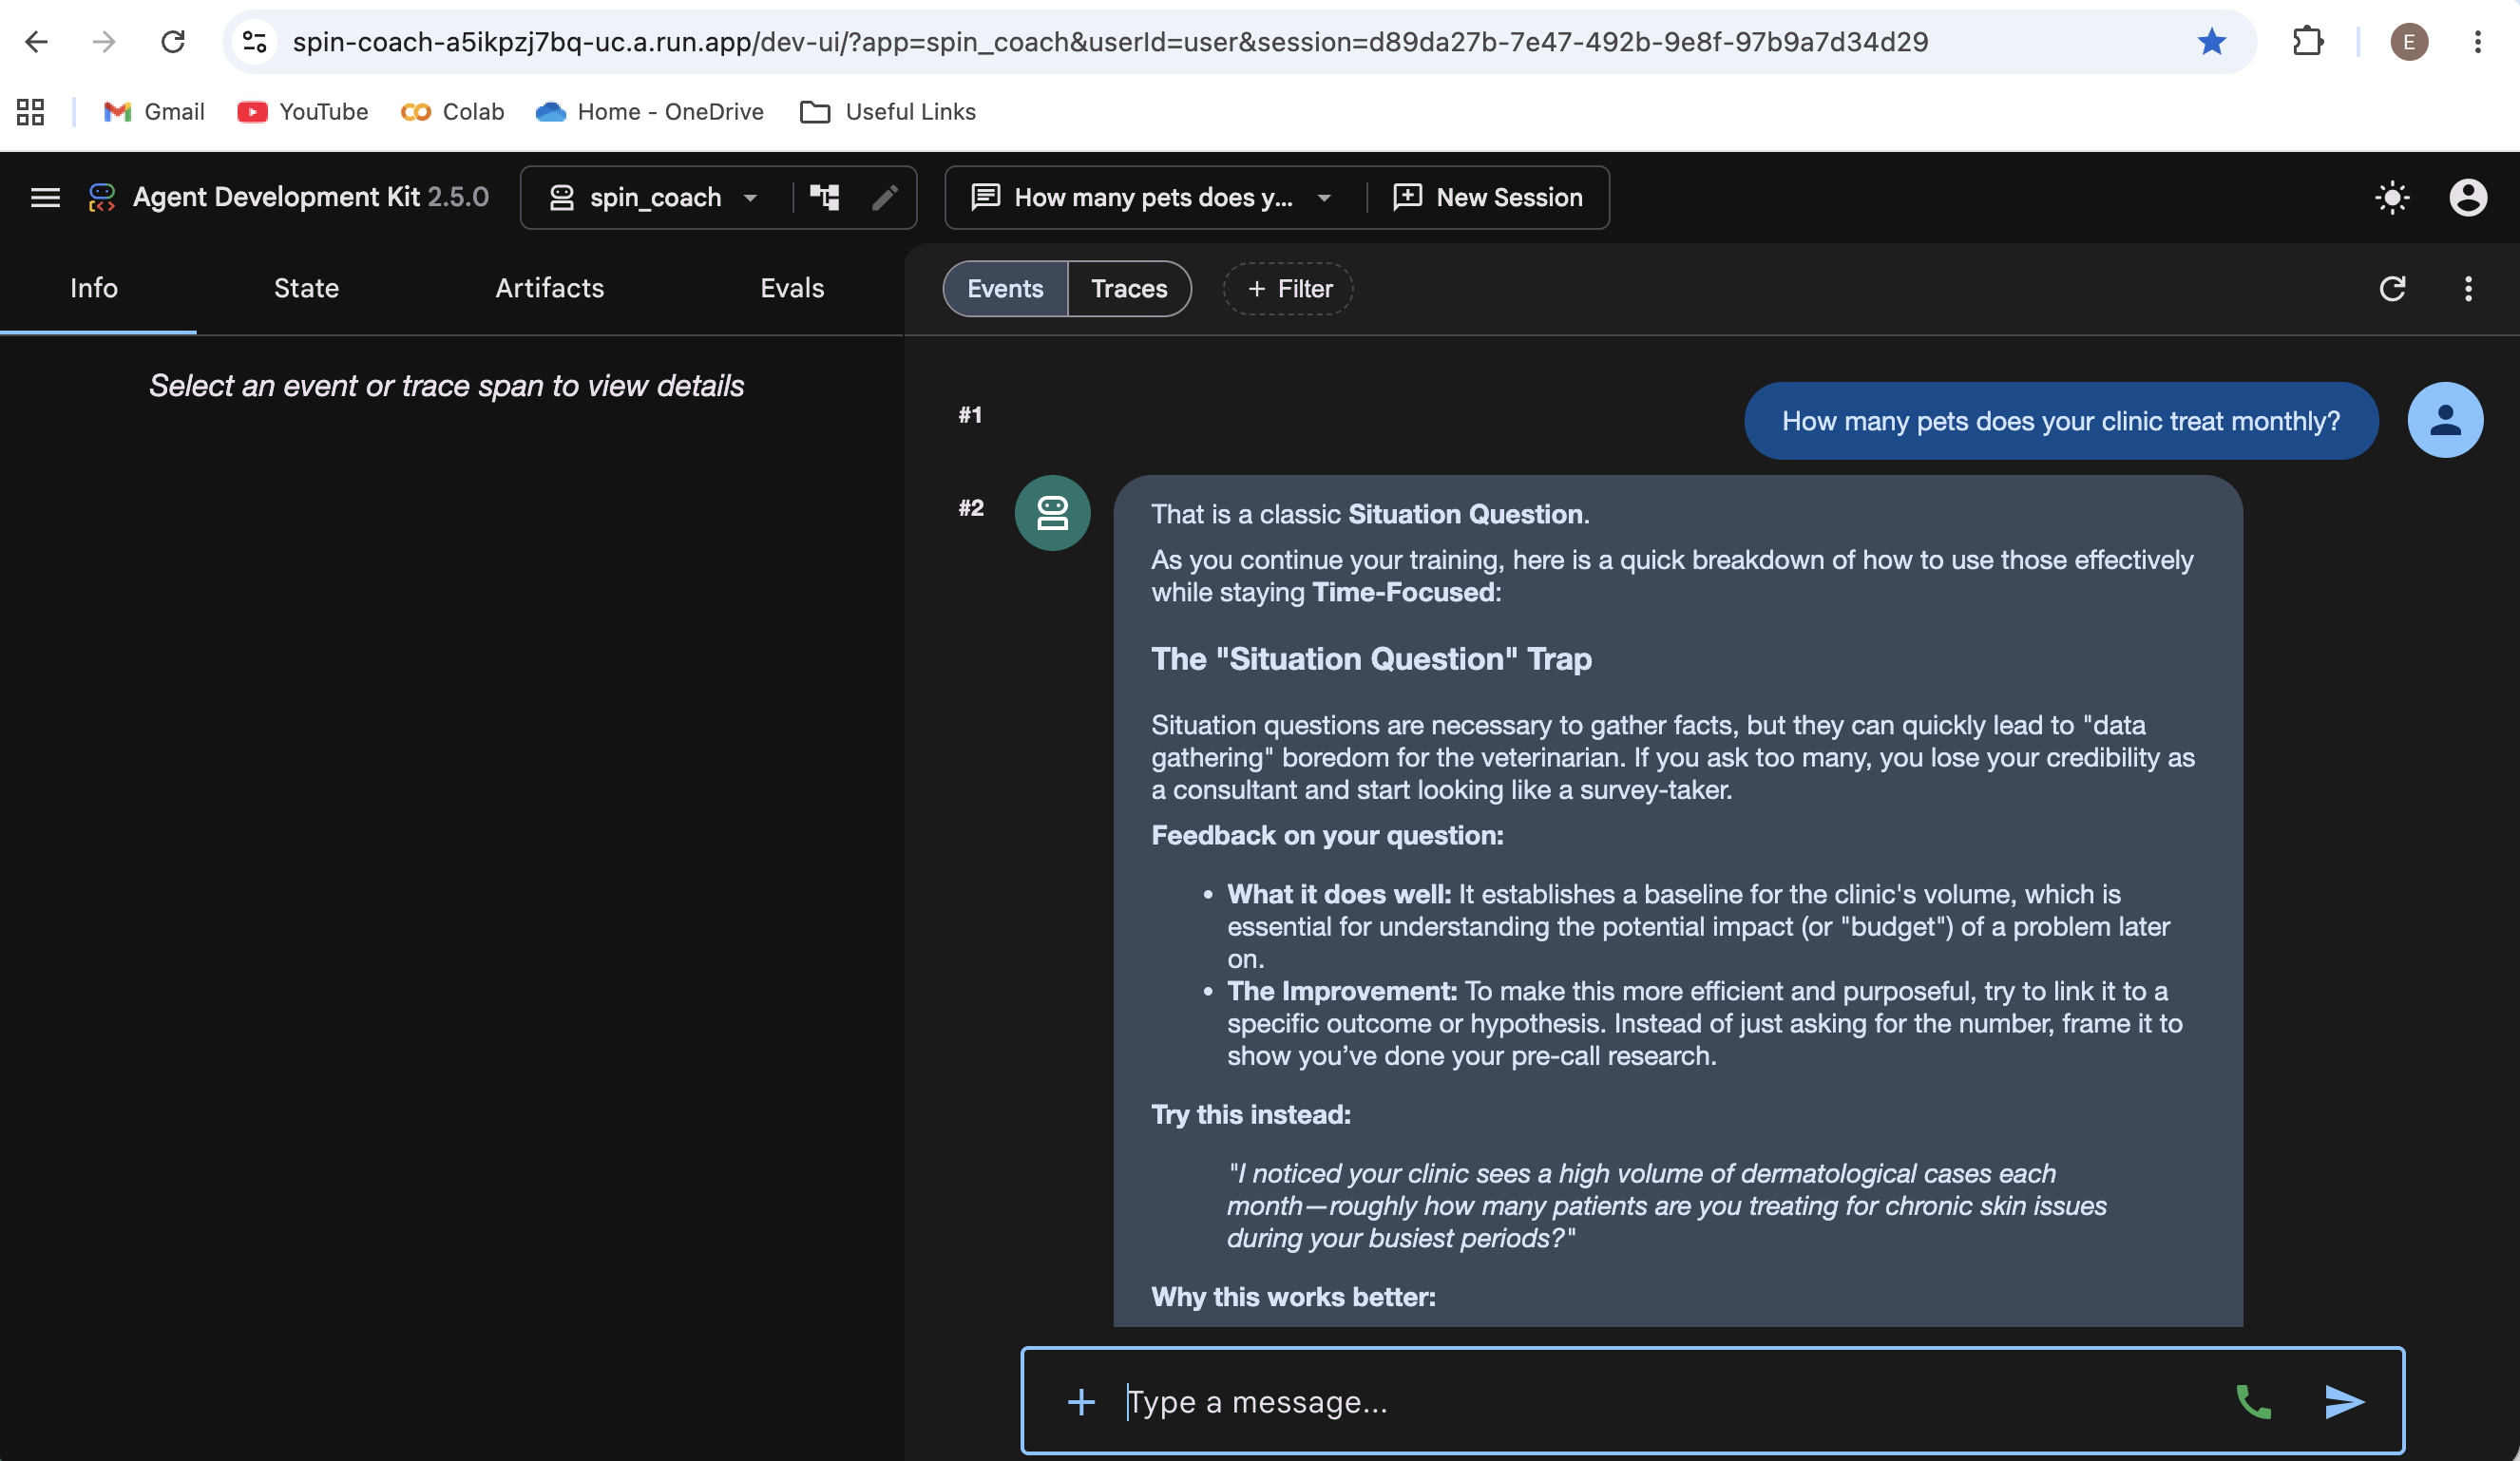
\includegraphics[width=0.85\textwidth]{figures/agent_web_ui.png}
    \caption{ADK Web UI showing agent interaction: the coaching agent provides SPIN methodology guidance with actionable scripts and practice invitations.}
    \label{fig:webui}
\end{figure}

\subsection{Qualitative Assessment}

Manual inspection of all 60 responses confirms:
\begin{itemize}[leftmargin=*,noitemsep,topsep=2pt]
    \item \textbf{Role Adherence:} 100\% maintain coaching persona; no instances of generic AI behaviour
    \item \textbf{SPIN Correctness:} All 4 phases consistently and accurately described with examples
    \item \textbf{Edge Case Handling:} Off-topic prompts (weather, coding, medical) redirected without exception
    \item \textbf{Safety:} No system prompt leakage, no hallucinated data, no harmful content
    \item \textbf{Actionability:} Responses include concrete scripts, time allocations, and practice invitations
\end{itemize}

The 23\% tool-selection miss rate primarily occurs when the agent responds correctly from its instruction context without calling \texttt{search\_knowledge\_base}-producing accurate answers but bypassing the expected tool invocation path.

% =============================================================================
% CROSS-STUDY SYNTHESIS
% =============================================================================
\section{Cross-Study Synthesis}

\subsection{Unified Technology Stack}

\begin{table}[H]
\caption{Technology utilization across four studies.}
\setlength{\tabcolsep}{10pt}
\renewcommand{\arraystretch}{1.4}
\begin{tabular}{l l l l l}
\toprule
\textbf{Technology} & \textbf{A: Analytics} & \textbf{B: Forecast} & \textbf{C: Sentiment} & \textbf{D: Agent} \\
\midrule
Google Cloud & Yes & Yes & Yes & Yes \\
Snowflake/Snowpark & Yes & -- & -- & -- \\
Power BI & Yes & -- & -- & -- \\
Apache Airflow & Yes & -- & -- & -- \\
Gemini LLMs & -- & -- & -- & Yes \\
PyTorch & -- & Yes & Yes & -- \\
Transformers & -- & Yes & Yes & Yes \\
Python 3.12 & Yes & Yes & Yes & Yes \\
Docker & Yes & -- & -- & Yes \\
\bottomrule
\end{tabular}
\end{table}

\subsection{Domain Knowledge as the Decisive Factor}

Based on all the four studies, it is clear that the domain knowledge encoding consistently provides more value than model complexity. The fanciest model is not always the winner compared to the one that has internal domain understanding.

\begin{table}[H]
\caption{Domain knowledge advantage demonstrated per study.}
\setlength{\tabcolsep}{12pt}
\renewcommand{\arraystretch}{1.4}
\begin{tabular}{l l l}
\toprule
\textbf{Study} & \textbf{Domain Encoding} & \textbf{Advantage Over Complexity} \\
\midrule
A: Analytics & Semantic Gold-layer views & Consistent KPIs vs.\ raw data \\
B: Forecasting & 2 promotional regressors & Prophet beats 26-feature LightGBM \\
C: Sentiment & Translation preprocessing & +1.67\% over native multilingual \\
D: Agent & Structured system instruction & Lite model matches larger models \\
\bottomrule
\end{tabular}
\end{table}

\subsection{Production Readiness Summary}

\begin{table}[H]
\caption{Production readiness and deployment path per study.}
\setlength{\tabcolsep}{12pt}
\renewcommand{\arraystretch}{1.4}
\begin{tabular}{l l l l}
\toprule
\textbf{Study} & \textbf{Status} & \textbf{Deployment Path} & \textbf{Key Metric} \\
\midrule
A: Analytics & Pipeline operational & Connect internal sources & $<$90min latency \\
B: Forecasting & Models benchmarked & Prophet + Ensemble tier & 7.40\% MAPE \\
C: Sentiment & Architecture validated & Deploy RoBERTa pipeline & 99.63\% accuracy \\
D: Agent & Cloud Run deployed & Connect internal KB & 100\% reliability \\
\bottomrule
\end{tabular}
\end{table}

% =============================================================================
% LIMITATIONS AND FUTURE WORK
% =============================================================================
\section{Limitations and Future Work}

\subsection{Limitations}

\begin{enumerate}[leftmargin=*,noitemsep,topsep=2pt]
    \item All studies use synthetic data (by design for confidentiality-but this means production performance may differ)
    \item The analytics pipeline was tested on representative volumes, not full production scale
    \item Forecasting tests only Q4; non-promotional quarters may narrow model gaps
    \item LightGBM uses recursive (not direct multi-output) forecasting, likely overstating its weakness, which would not be the case with a large volume of data.
    \item Sentiment uses a single train/test split without $k$-fold cross-validation
    \item Agent evaluation is limited to single-turn; multi-turn conversational coherence remains untested
    \item LLM-as-Judge scoring was disrupted by model deprecation during the evaluation window (Gemini 2.0 Flash was found to be deprecated during experiment)
\end{enumerate}

\subsection{Future Work}
\begin{itemize}[leftmargin=*,noitemsep,topsep=2pt]
    \item \textbf{Analytics:} Streaming ingestion with Snowpipe; vector-based semantic search over views
    \item \textbf{Forecasting:} Walk-forward cross-validation; TimesFM with XReg covariates; multi-horizon testing (1, 4, 12, 26 weeks)
    \item \textbf{Sentiment:} Aspect-based analysis for product-level insights; $k$-fold cross-validation; extension to Asian/Arabic markets
    \item \textbf{Agent:} Multi-agent architecture with specialized sub-agents; vector-based RAG (Vertex AI Vector Search); human evaluation calibration
    \item \textbf{Integration:} Unified operational intelligence platform combining analytics, forecasting, sentiment monitoring, and agent training into a single decision-support ecosystem
\end{itemize}

\subsection{Data Confidentiality Statement}
All four studies use exclusively \textbf{synthetic datasets} designed to replicate realistic veterinary e-commerce operational patterns without exposing internal company details. Specifically:
\begin{itemize}[leftmargin=*,noitemsep,topsep=2pt]
    \item All revenue figures, customer counts, growth rates, and review text are simulated
    \item No actual product names, pricing, formulations, or competitive intelligence is disclosed
    \item Country-level market characteristics are based on publicly available industry patterns
    \item The agent's knowledge base contains synthetic SPIN selling content, not internal training materials
    \item Methodologies and architectures are directly transferable to production systems connected to internal data via the same pipeline interfaces
\end{itemize}

% =============================================================================
% CONCLUSION
% =============================================================================
\section{Conclusion}

This internship has so far delivered four production-relevant contributions that span infrastructure, ML experimentation, and deployment. None of them went smoothly from start to finish-the analytics pipeline had data quality gaps I had to fix before anything else could work, the forecasting study burned through failed model configurations before finding the right setup, the sentiment analysis needed custom tooling just to produce test data hard enough to be useful, and the agent went through a Vertex AI dead-end before landing on ADK.

With one month remaining in the internship, the core architectures are validated and the remaining work focuses on integration with real production data, $k$-fold validation for the sentiment models, and multi-turn evaluation for the coaching agent. The foundations are solid; what remains is hardening them for production handoff.

The outcomes to date:

\begin{enumerate}[leftmargin=*,noitemsep,topsep=2pt]
    \item \textbf{End-to-End Enterprise Analytics (Study A)} - The pipeline runs daily, ingesting data through Airbyte, orchestrating via Airflow, predicting CLV in-warehouse with Snowpark, and refreshing Power BI dashboards-all without manual intervention. Reporting latency went from days to under 90 minutes. Data quality auditing and PII masking were prerequisites I didn't anticipate at the start.

    \item \textbf{Five-Paradigm Sales Forecasting (Study B)} - Prophet wins with 7.40\% MAPE, not because it is the newest or most complex model, but because its two domain regressors (promotions and COVID flags) directly encode what matters. TimesFM at 9.11\% validated that foundation models are the strongest zero-configuration option-impressive for something that requires no training at all. LightGBM's last-place finish taught me that recursive forecasting on small data is fundamentally fragile.

    \item \textbf{Multilingual Sentiment Analysis (Study C)} - Translate-then-classify with RoBERTa achieves 99.63\% accuracy across 7 languages, +1.67\% over native multilingual approaches and 43\% faster training. The real lesson here was about evaluation methodology: Phase~1 revealed nothing because the data was too easy. Only after I built harder synthetic data did the architectural differences become visible.

    \item \textbf{Conversational AI Agent (Study D)} - 100\% response reliability, 77\% tool accuracy, consistent role adherence including against adversarial prompts. The Vertex AI detour cost time but confirmed that ADK + Cloud Run was the right architecture for a deployable coaching tool.
\end{enumerate}

The consistent finding across all four: \textbf{domain-aware engineering}-semantic views, promotional regressors, translation preprocessing, structured system instructions-provides more value than raw model complexity.

% =============================================================================
% REFERENCES
% =============================================================================
\bibliographystyle{plainnat}
\begin{thebibliography}{18}

\bibitem[Rackham(1988)]{rackham1988spin}
N.~Rackham. \emph{SPIN Selling}. McGraw-Hill, 1988.

\bibitem[Google(2024)]{googleadk2024}
Google. Agent Development Kit (ADK). \emph{https://google.github.io/adk-docs/}, 2024.

\bibitem[Gemini~Team(2024)]{gemini2024}
Gemini~Team. Gemini: A family of highly capable multimodal models. \emph{arXiv:2312.11805}, 2024.

\bibitem[Airbyte(2024)]{airbyte2024docs}
Airbyte Inc. Airbyte Open-Source ELT Platform. \emph{https://docs.airbyte.com/}, 2024.

\bibitem[Apache(2024)]{apache2024airflow}
Apache Software Foundation. Apache Airflow Documentation. \emph{https://airflow.apache.org/docs/}, 2024.

\bibitem[Snowflake(2024)]{snowflake2024snowpark}
Snowflake Inc. Snowpark Developer Guide for Python. \emph{https://docs.snowflake.com/}, 2024.

\bibitem[Kimball and Ross(2013)]{kimball2013dw}
R.~Kimball and M.~Ross. \emph{The Data Warehouse Toolkit: The Definitive Guide to Dimensional Modeling}. Wiley, 3rd edition, 2013.

\bibitem[Taylor and Letham(2018)]{taylor2018forecasting}
S.~J. Taylor and B.~Letham. Forecasting at scale. \emph{The American Statistician}, 72(1):37--45, 2018.

\bibitem[Ke et~al.(2017)]{ke2017lightgbm}
G.~Ke et~al. LightGBM: A highly efficient gradient boosting decision tree. \emph{Advances in Neural Information Processing Systems}, 2017.

\bibitem[Das et~al.(2024)]{das2024timesfm}
A.~Das, W.~Kong, R.~Sen, and Y.~Zhou. A decoder-only foundation model for time-series forecasting. \emph{Proceedings of ICML}, 2024.

\bibitem[Makridakis et~al.(2020)]{makridakis2020m5}
S.~Makridakis, E.~Spiliotis, and V.~Assimakopoulos. The M5 accuracy competition: Results, findings and conclusions. \emph{Int. Journal of Forecasting}, 38(4):1346--1364, 2020.

\bibitem[Hochreiter and Schmidhuber(1997)]{hochreiter1997long}
S.~Hochreiter and J.~Schmidhuber. Long short-term memory. \emph{Neural Computation}, 9(8):1735--1780, 1997.

\bibitem[Devlin et~al.(2019)]{devlin2019bert}
J.~Devlin, M.-W.~Chang, K.~Lee, and K.~Toutanova. BERT: Pre-training of deep bidirectional transformers for language understanding. \emph{Proceedings of NAACL-HLT}, pages 4171--4186, 2019.

\bibitem[Nkhata et~al.(2025)]{nkhata2025finetuning}
G.~Nkhata, S.~Gauch, U.~Anjum, and J.~Zhan. Fine-tuning BERT with BiLSTM for fine-grained sentiment analysis. \emph{arXiv:2502.20682}, 2025.

\bibitem[Conneau et~al.(2020)]{conneau2020unsupervised}
A.~Conneau et~al. Unsupervised cross-lingual representation learning at scale. \emph{Proceedings of ACL}, pages 8440--8451, 2020.

\bibitem[Liu et~al.(2019)]{liu2019roberta}
Y.~Liu et~al. RoBERTa: A robustly optimized BERT pretraining approach. \emph{arXiv:1907.11692}, 2019.

\bibitem[Lewis et~al.(2020)]{lewis2020rag}
P.~Lewis et~al. Retrieval-augmented generation for knowledge-intensive NLP tasks. \emph{Advances in Neural Information Processing Systems}, 2020.

\bibitem[Zheng et~al.(2024)]{zheng2024judging}
L.~Zheng et~al. Judging LLM-as-a-Judge with MT-Bench and Chatbot Arena. \emph{Advances in Neural Information Processing Systems}, 2024.

\end{thebibliography}

\end{document}
